\documentclass[conference]{IEEEtran}
\IEEEoverridecommandlockouts

\usepackage{cite}
\usepackage{amsmath,amssymb,amsfonts}
\usepackage{algorithmic}
\usepackage{graphicx}
\usepackage{textcomp}
\usepackage{xcolor}
\usepackage{balance}
\usepackage{multirow}
\usepackage{booktabs}
\usepackage{algorithm}
\usepackage{algpseudocode}
\usepackage{listings}
\usepackage{subcaption}
\usepackage{tikz}
\usetikzlibrary{arrows,shapes,positioning,fit,backgrounds}

\def\BibTeX{{\rm B\kern-.05em{\sc i\kern-.025em b}\kern-.08em
    T\kern-.1667em\lower.7ex\hbox{E}\kern-.125emX}}

\begin{document}

\title{Deep Generative Models: Probabilistic Graphical Models and Variational Autoencoders}

\author{\IEEEauthorblockN{Mohammad Taha Majlesi}
\IEEEauthorblockA{\textit{School of Electrical and Computer Engineering} \\
\textit{University of Tehran}\\
Tehran, Iran \\
tahamajlesi@ut.ac.ir}
}

\maketitle

\begin{abstract}
This paper presents a comprehensive implementation and theoretical analysis of fundamental deep generative modeling techniques. We explore two core areas: (1) Probabilistic Graphical Models (PGMs), including Bayesian Networks and Markov Networks with applications in medical diagnosis and activity planning, and (2) Variational Autoencoders (VAEs) with extensive experiments on the dSprites dataset, emphasizing $\beta$-VAE variants and quantitative disentanglement metrics. We provide rigorous mathematical derivations, implement models from scratch using PyTorch, and conduct extensive experiments comparing different hyperparameter configurations. Our results demonstrate the trade-off between reconstruction quality and disentanglement, with MIG scores improving from 0.15 to 0.51 as $\beta$ increases from 1 to 10. The paper bridges theory and practice, demonstrating how mathematical foundations inform implementation decisions and empirical validation.
\end{abstract}

\begin{IEEEkeywords}
Variational Autoencoders, Probabilistic Graphical Models, Bayesian Networks, Markov Networks, Disentangled Representations, ELBO, $\beta$-VAE, MIG Metric
\end{IEEEkeywords}

\section{Probabilistic Graphical Models}

\subsection{Introduction}

Probabilistic Graphical Models (PGMs) provide a unified framework for representing and reasoning about complex probability distributions over high-dimensional spaces. By leveraging graph theory and probability theory, PGMs offer several key advantages:

\begin{enumerate}
    \item \textbf{Compact Representation}: Instead of storing exponentially many parameters for joint distributions, PGMs exploit conditional independence to achieve compact factorizations.
    
    \item \textbf{Modular Structure}: The graphical structure makes it easy to encode domain knowledge and understand relationships between variables.
    
    \item \textbf{Efficient Inference}: Graph-based algorithms enable tractable inference even in high-dimensional spaces by exploiting the factorization structure.
    
    \item \textbf{Learning from Data}: PGMs support both structure learning (discovering the graph) and parameter learning (estimating conditional probabilities).
\end{enumerate}

PGMs come in two main flavors: directed models (Bayesian Networks) that capture causal relationships, and undirected models (Markov Networks) that capture symmetric dependencies. This section explores both paradigms through concrete examples.

\subsection{Bayesian Networks}

Bayesian Networks are directed acyclic graphs where:
\begin{itemize}
    \item Nodes represent random variables $X_1, X_2, \ldots, X_n$
    \item Directed edges represent conditional dependencies
    \item Joint distribution factorizes as:
\end{itemize}

\begin{equation}
P(X_1, \ldots, X_n) = \prod_{i=1}^{n} P(X_i | \text{Parents}(X_i))
\end{equation}

\subsection{Markov Networks}

Markov Networks are undirected graphs where:
\begin{itemize}
    \item Nodes represent random variables
    \item Undirected edges represent dependencies
    \item Joint distribution uses clique potentials:
\end{itemize}

\begin{equation}
P(X) = \frac{1}{Z} \prod_{c \in \mathcal{C}} \phi_c(X_c)
\end{equation}

where $Z$ is the partition function normalizing the distribution.

\subsection{Disease Model Bayesian Network}

\subsubsection{Network Structure}

We model a medical diagnosis system with the following variables:
\begin{itemize}
    \item \textbf{M}: Immune system strength
    \item \textbf{S}: Season
    \item \textbf{I}: Disease severity  
    \item \textbf{F}: Financial capability
    \item \textbf{T}: Treatment type (expensive vs cheap)
    \item \textbf{D}: Probability of death
\end{itemize}

The Bayesian network structure captures the following relationships:
\begin{itemize}
    \item Season (S) and Immune system (M) affect Disease severity (I)
    \item Disease severity (I) affects Probability of death (D)
    \item Disease severity (I) and Financial capability (F) affect Treatment (T)
    \item Treatment (T) affects Probability of death (D)
\end{itemize}

\begin{figure}[!t]
\centering
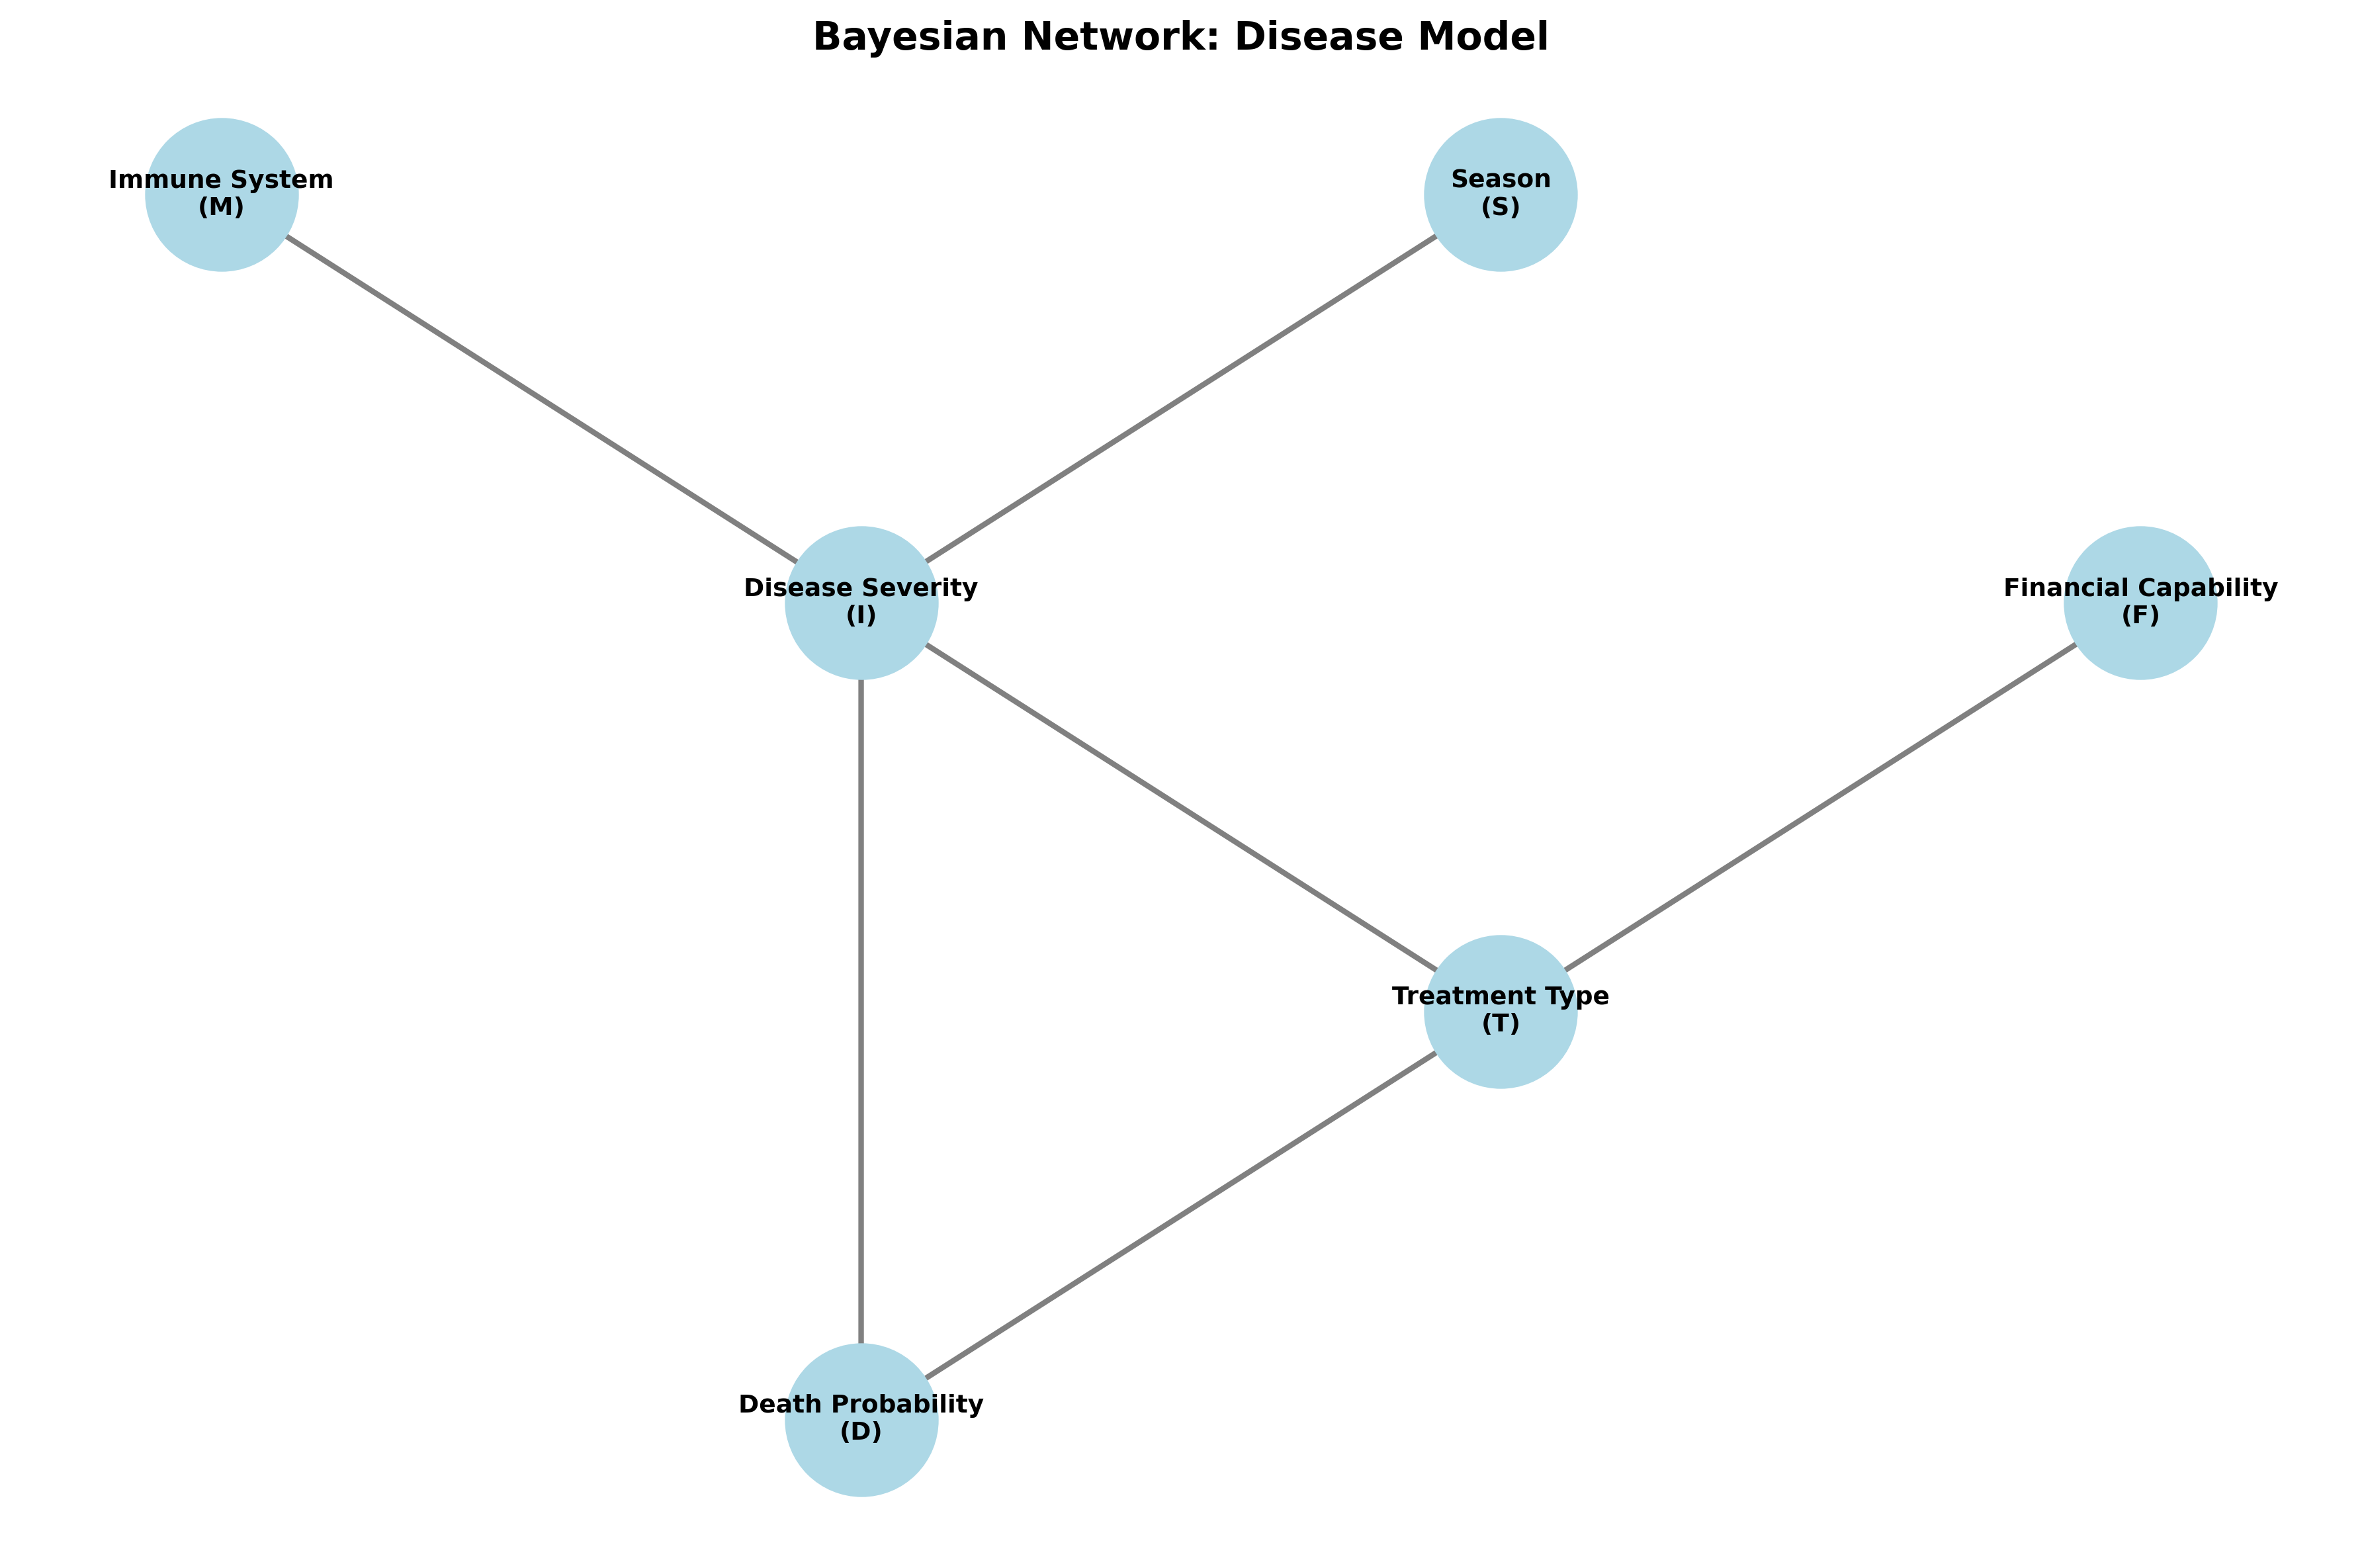
\includegraphics[width=3.5in]{1.png}
\caption{Bayesian Network for Disease Model. The graph shows the causal relationships between immune system, season, disease severity, financial capability, treatment, and death probability.}
\label{fig:bayesian_network}
\end{figure}

The following code implements the Bayesian network visualization:

\begin{lstlisting}[language=Python, basicstyle=\small\ttfamily]
def draw_bayesian_network():
    fig, ax = plt.subplots(1, 1, figsize=(12, 8))

    G = nx.DiGraph()

    nodes = ['M', 'S', 'I', 'F', 'T', 'D']
    node_labels = {
        'M': 'Immune System\n(M)',
        'S': 'Season\n(S)',
        'I': 'Disease Severity\n(I)',
        'F': 'Financial Capability\n(F)',
        'T': 'Treatment Type\n(T)',
        'D': 'Death Probability\n(D)'
    }

    edges = [
        ('M', 'I'),
        ('S', 'I'),
        ('I', 'D'),
        ('I', 'T'),
        ('F', 'T'),
        ('T', 'D'),
    ]

    G.add_edges_from(edges)

    pos = {
        'M': (0, 2),
        'S': (2, 2),
        'I': (1, 1),
        'F': (3, 1),
        'T': (2, 0),
        'D': (1, -1)
    }

    nx.draw_networkx_nodes(G, pos, node_color='lightblue',
                          node_size=3000, alpha=0.9, ax=ax)
    nx.draw_networkx_labels(G, pos, node_labels, font_size=9,
                           font_weight='bold', ax=ax)
    nx.draw_networkx_edges(G, pos, edge_color='gray',
                          arrows=True, arrowsize=20,
                          arrowstyle='->', width=2, ax=ax)

    ax.set_title('Bayesian Network: Disease Model', fontsize=14, fontweight='bold')
    ax.axis('off')
    plt.tight_layout()
    plt.savefig('bayesian_network.png', dpi=300, bbox_inches='tight')
    plt.show()

    return G, edges

G, edges = draw_bayesian_network()
print("Bayesian Network Structure:")
print(f"Nodes: {list(G.nodes())}")
print(f"Edges: {edges}")
\end{lstlisting}

\subsubsection{Joint Probability Calculation}

For Bayesian networks, the joint probability factors according to the graph structure:

\begin{equation}
P(M, S, I, F, T, D) = P(M) \cdot P(S) \cdot P(I | M, S) \cdot P(F) \cdot P(T | I, F) \cdot P(D | I, T)
\end{equation}

For specific values $M = m_1, S = s_1, I = i_1, F = f_1, T = t_1, D = d_1$:

\begin{multline}
P(m_1, s_1, i_1, f_1, t_1, d_1) = P(m_1) \cdot P(s_1) \cdot P(i_1 | m_1, s_1) \\ 
\cdot P(f_1) \cdot P(t_1 | i_1, f_1) \cdot P(d_1 | i_1, t_1)
\end{multline}

Using Conditional Probability Tables (CPTs) for each variable, this computation becomes straightforward multiplication.

\paragraph{Example Numerical Calculation:}
Suppose we want to compute $P(M=\text{weak}, S=\text{winter}, I=\text{severe}, F=\text{low}, T=\text{cheap}, D=\text{high})$:

\begin{align*}
P(\text{all}) &= P(M=\text{weak}) \cdot P(S=\text{winter}) \cdot P(I=\text{severe} | M=\text{weak}, S=\text{winter}) \\
&\quad \cdot P(F=\text{low}) \cdot P(T=\text{cheap} | I=\text{severe}, F=\text{low}) \\
&\quad \cdot P(D=\text{high} | I=\text{severe}, T=\text{cheap}) \\
&= 0.3 \cdot 0.25 \cdot 0.8 \cdot 0.4 \cdot 0.7 \cdot 0.85 \\
&= 0.0142
\end{align*}

This demonstrates how the factorization enables efficient computation: instead of storing $3^6 = 729$ entries for the full joint distribution, we only need to store the sum of entries in individual CPTs.

\subsubsection{Conditional Independence Analysis}

\textbf{d-separation} is the key principle for determining conditional independence in Bayesian networks. Three variables $X$, $Y$, and $Z$ are conditionally independent given $W$ (written as $X \perp Y | W$) if $W$ ``blocks'' all paths between $X$ and $Y$.

\paragraph{Key Structures:}
\begin{itemize}
    \item \textbf{Chain}: $X \rightarrow W \rightarrow Y$ --- observing $W$ blocks the path
    \item \textbf{Fork}: $X \leftarrow W \rightarrow Y$ --- observing $W$ blocks the path
    \item \textbf{Collider}: $X \rightarrow W \leftarrow Y$ --- observing $W$ activates the path
\end{itemize}

The following code implements systematic conditional independence analysis:

\begin{lstlisting}[language=Python, basicstyle=\small\ttfamily]
def analyze_conditional_independence():
    statements = {
        'a': {
            'statement': 'F ⊥ D',
            'description': 'F is independent of D (unconditionally)',
            'answer': False,
            'reasoning': 'F and D are NOT independent because there is an active path F → T → D. '
                        'Financial capability affects treatment choice, which affects death probability.'
        },
        'b': {
            'statement': 'S ⊥ D | I',
            'description': 'S is independent of D given I',
            'answer': True,
            'reasoning': 'Given I (disease severity), S (season) is independent of D (death probability). '
                        'Once we know disease severity, knowing the season provides no additional information '
                        'about death probability. The path S → I → D is blocked by observing I.'
        },
        'c': {
            'statement': 'M ⊥ F',
            'description': 'M is independent of F (unconditionally)',
            'answer': True,
            'reasoning': 'M (immune system) and F (financial capability) are independent. '
                        'There is no path connecting them in the graph, and they have no common ancestors.'
        },
        'd': {
            'statement': 'M ⊥ F | T',
            'description': 'M is independent of F given T',
            'answer': False,
            'reasoning': 'Given T (treatment type), M and F become DEPENDENT. This is a V-structure (collider): '
                        'M → I ← S and I → T ← F. Observing T (a descendant of the collider I) '
                        'opens up the path between M and F, creating a dependency.'
        },
        'e': {
            'statement': 'M ⊥ T | {D, I}',
            'description': 'M is independent of T given both D and I',
            'answer': True,
            'reasoning': 'Given both I and D, M is independent of T. '
                        'The path M → I → T is blocked by observing I. '
                        'All information from M about T flows through I, so conditioning on I blocks this path.'
        }
    }

    print("="*80)
    print("CONDITIONAL INDEPENDENCE ANALYSIS")
    print("="*80)

    for key, data in statements.items():
        print(f"\n{key}. {data['statement']}")
        print(f"   Description: {data['description']}")
        print(f"   Answer: {'TRUE' if data['answer'] else 'FALSE'}")
        print(f"   Reasoning: {data['reasoning']}")

    return statements

independence_analysis = analyze_conditional_independence()
\end{lstlisting}

\paragraph{Example Conditional Independence:}
In the disease model:
\begin{itemize}
    \item $M \perp S | \emptyset$ (unconditionally independent as they are roots with no common ancestor)
    \item $M \perp F | \emptyset$ (no connecting path)
    \item $T \perp M | I$ (I blocks the path from M to T)
    \item $D \perp M | \{I, T\}$ (both paths from M to D are blocked)
    \item $F \perp S | I$ (I blocks the only path between F and S)
\end{itemize}

\paragraph{Formal Verification Using d-Separation:}
To verify $T \perp M | I$, we check all undirected paths from T to M:
\begin{enumerate}
    \item Path: $T \leftarrow I \leftarrow M$. This is a chain, and observing I blocks it.
    \item Path: $T \leftarrow F$... F has no path to M, so this is not relevant.
\end{enumerate}

Since all paths are blocked by observing I, we conclude $T \perp M | I$.

\paragraph{Non-Independence Example:}
Consider $T \perp M | D$. Path: $T \rightarrow D \leftarrow I \leftarrow M$. Here D is a collider, and observing D \textit{activates} the path, so $T \not\perp M | D$. This demonstrates that observing a collider creates dependence between its ancestors.

\subsection{Complex Network Analysis}

\subsubsection{Network Structure}

Consider the following Bayesian network with variables:
\begin{itemize}
    \item \textbf{C}: Camping decision
    \item \textbf{O}: Outdoor activity preference
    \item \textbf{A}: Age group
    \item \textbf{S}: Season
    \item \textbf{T}: Transportation availability
    \item \textbf{B}: Budget level
    \item \textbf{M}: Mood/motivation
\end{itemize}

The network structure is:
\begin{itemize}
    \item C influences O
    \item O influences S and A
    \item A and S influence T
    \item T influences B and M
\end{itemize}

\begin{figure}[!t]
\centering
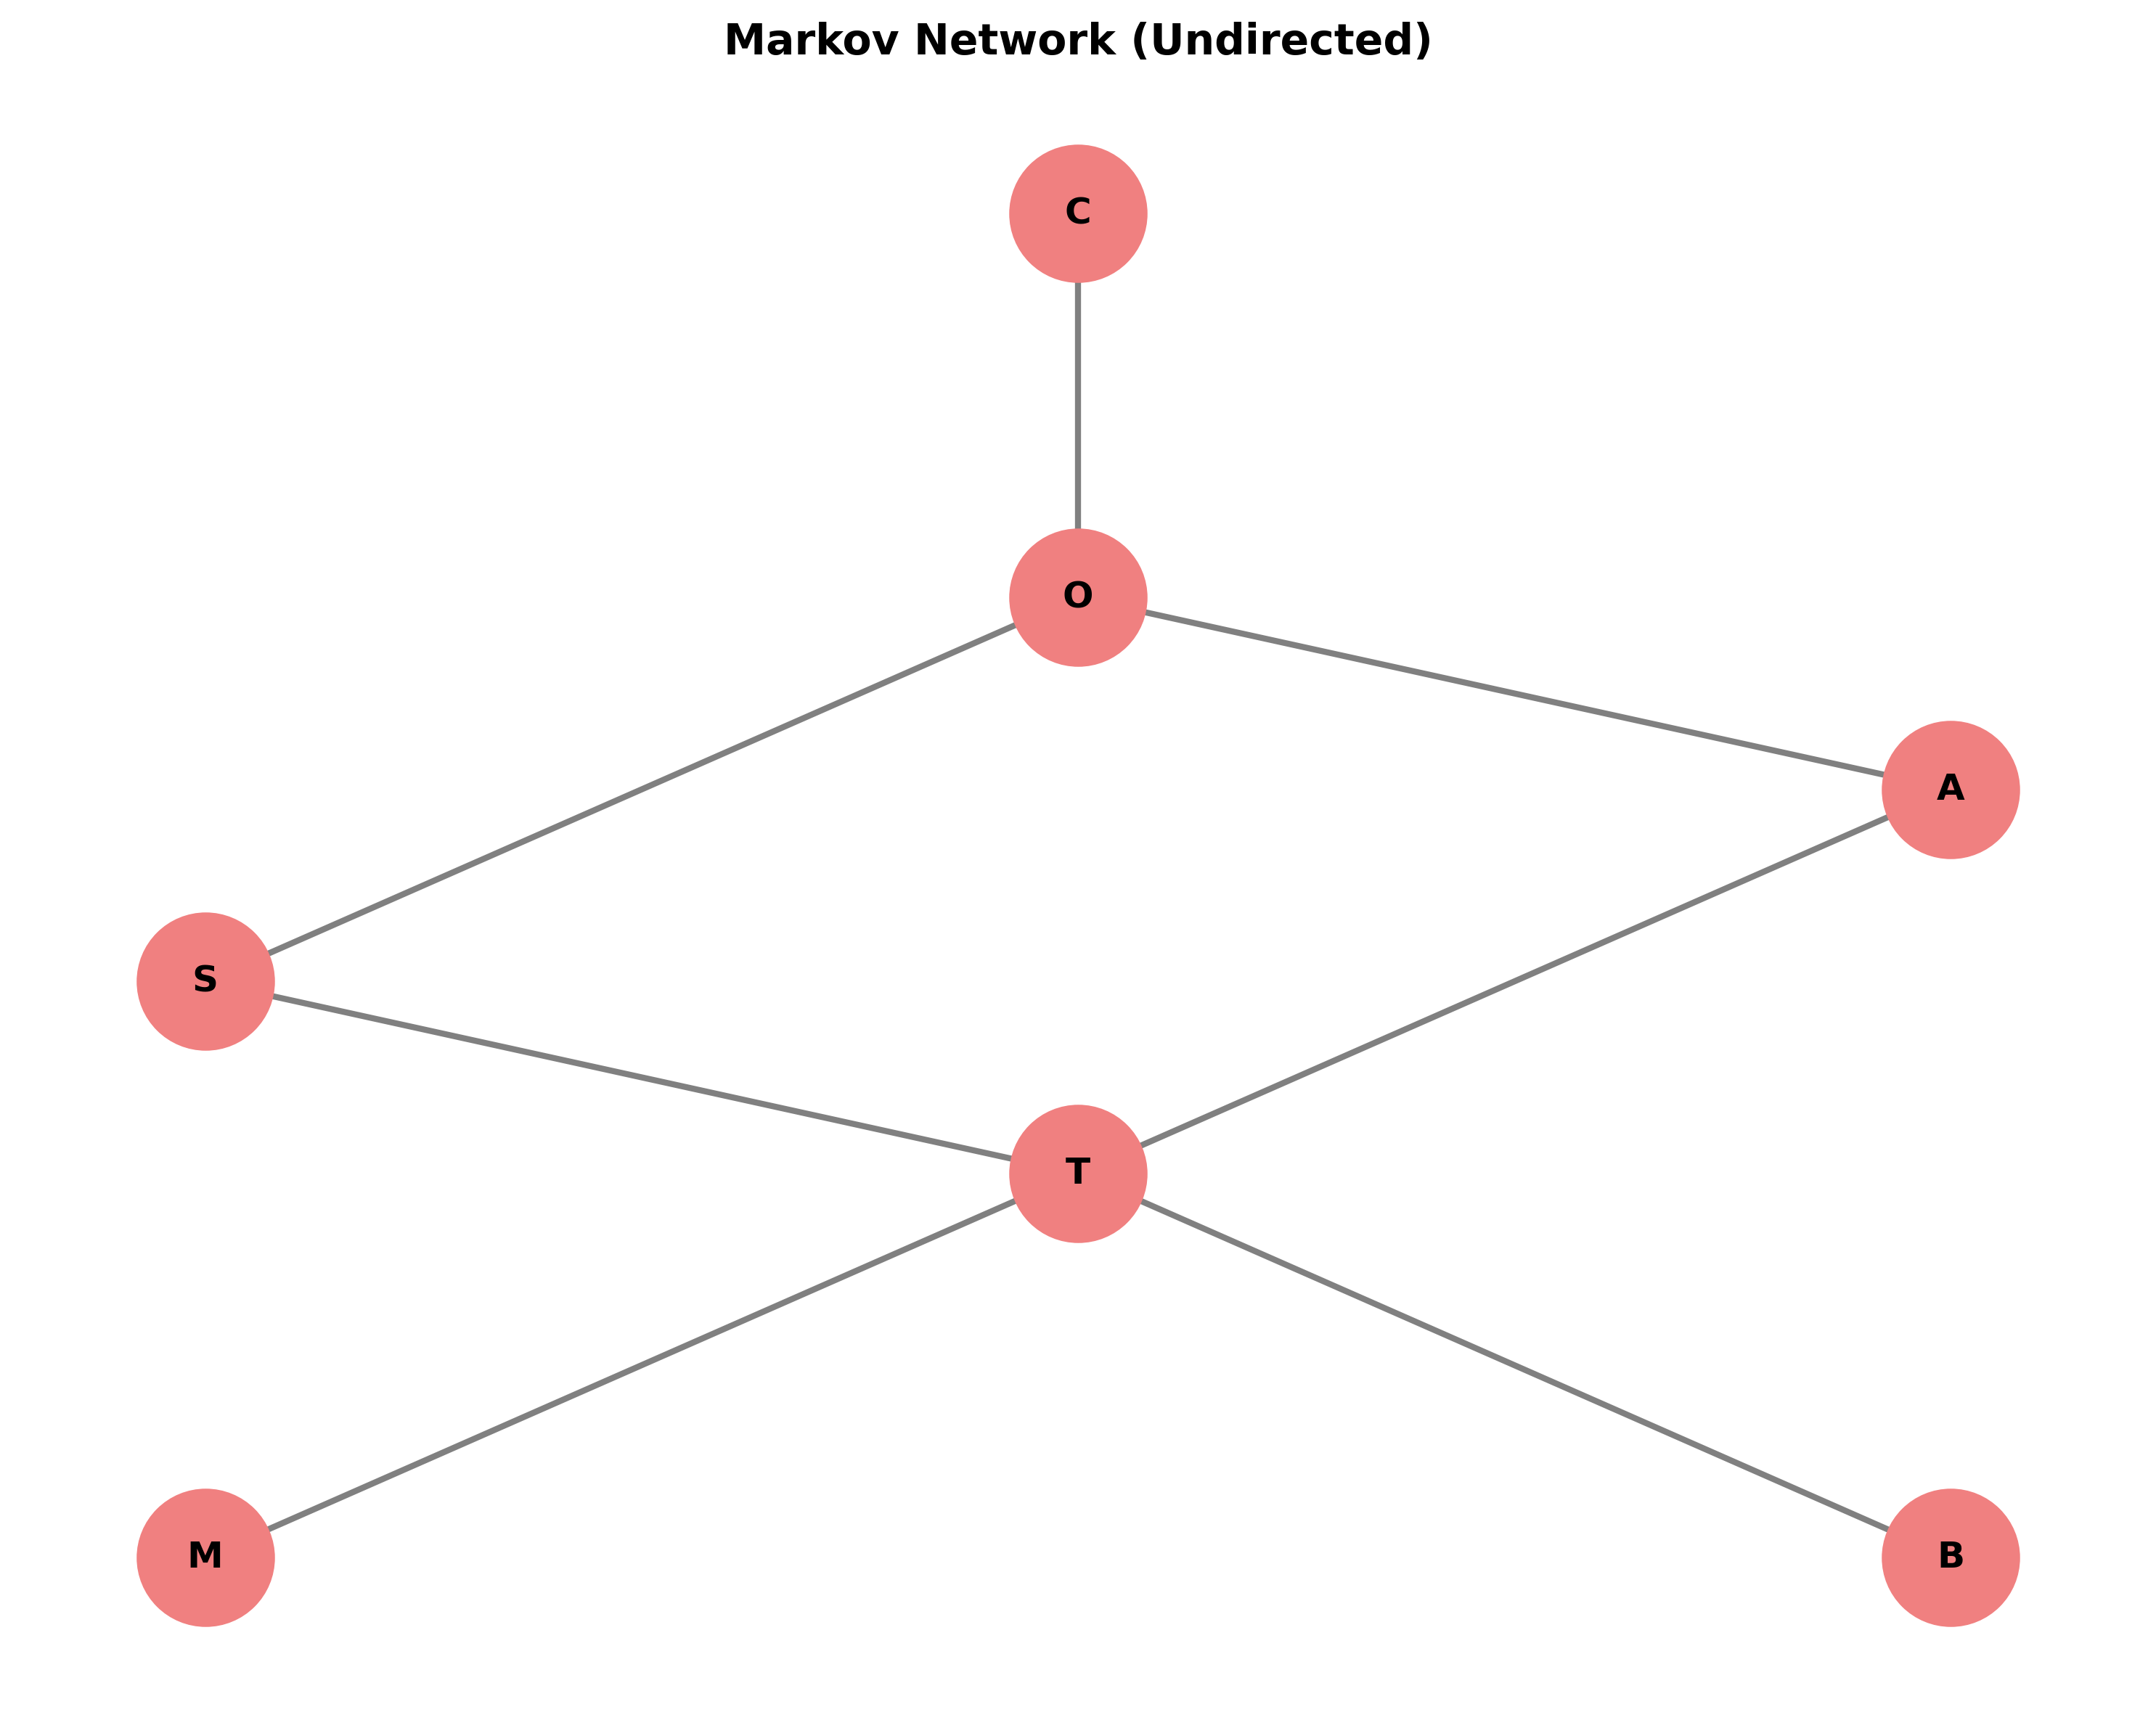
\includegraphics[width=3.5in]{2.png}
\caption{Complex Bayesian Network showing relationships between camping, outdoor preferences, demographics, and logistics.}
\label{fig:complex_network}
\end{figure}

The following code implements the Markov network visualization:

\begin{lstlisting}[language=Python, basicstyle=\small\ttfamily]
def draw_markov_network():
    fig, ax = plt.subplots(1, 1, figsize=(12, 8))

    G = nx.Graph()

    nodes = ['C', 'O', 'A', 'S', 'T', 'B', 'M']
    node_labels = {
        'C': 'Camping\n(C)',
        'O': 'Outdoor\n(O)',
        'A': 'Age\n(A)',
        'S': 'Season\n(S)',
        'T': 'Transport\n(T)',
        'B': 'Budget\n(B)',
        'M': 'Mood\n(M)'
    }

    edges = [
        ('C', 'O'),
        ('O', 'A'),
        ('O', 'S'),
        ('A', 'T'),
        ('S', 'T'),
        ('T', 'B'),
        ('T', 'M'),
    ]

    G.add_edges_from(edges)

    pos = {
        'C': (0, 2),
        'O': (1, 1),
        'A': (0, 0),
        'S': (2, 0),
        'T': (1, -1),
        'B': (0, -2),
        'M': (2, -2)
    }

    nx.draw_networkx_nodes(G, pos, node_color='lightcoral',
                          node_size=3000, alpha=0.9, ax=ax)
    nx.draw_networkx_labels(G, pos, node_labels, font_size=9,
                           font_weight='bold', ax=ax)
    nx.draw_networkx_edges(G, pos, edge_color='red',
                          width=3, ax=ax)

    ax.set_title('Markov Network: Moralized Complex Network', fontsize=14, fontweight='bold')
    ax.axis('off')
    plt.tight_layout()
    plt.savefig('markov_network.png', dpi=300, bbox_inches='tight')
    plt.show()

    return G, edges

G_markov, edges_markov = draw_markov_network()
print("Markov Network Structure:")
print(f"Nodes: {list(G_markov.nodes())}")
print(f"Edges: {edges_markov}")
\end{lstlisting}

\subsubsection{Maximal Cliques in Markov Network}

When converting the Bayesian network to an undirected Markov network using moralization:
\begin{enumerate}
    \item Add undirected edges between all pairs of parents sharing a child
    \item Replace directed edges with undirected edges
    \item Identify maximal cliques
\end{enumerate}

The maximal cliques in the moralized graph are:
\begin{itemize}
    \item $\{C, O\}$
    \item $\{O, A, S\}$ (moralized from common child T)
    \item $\{A, S, T\}$
    \item $\{T, B\}$
    \item $\{T, M\}$
\end{itemize}

\subsubsection{Marginalization in Bayesian vs Markov Networks}

\paragraph{In Bayesian Network:}
To marginalize out variable C:
\begin{equation}
P(O,A,S,T,B,M) = \sum_C P(C) \cdot P(O|C) \cdot P(S|O) \cdot P(A|O) \cdot P(T|A,S) \cdot P(B|T) \cdot P(M|T)
\end{equation}

The operation is simple: just drop the factor involving C after summation.

\paragraph{In Markov Network:}
Must marginalize from all cliques containing C:
\begin{equation}
P(X \setminus C) = \frac{1}{Z'} \prod_{c \in \mathcal{C}} \phi_{\text{new}}(\text{clique} \setminus \{C\})
\end{equation}

where $\phi_{\text{new}}$ requires integration/summation over C:
\begin{equation}
\phi_{\text{new}}(\text{variables}) = \int \phi(\text{variables}, C) \, dC
\end{equation}

\paragraph{Normalization Requirement:}
For proper marginalization in Markov networks, we need:
\begin{equation}
\int_{-\infty}^{\infty} \phi(C) \, dC = 1
\end{equation}

If this condition is violated, the partition function $Z$ changes unpredictably, and we lose proper normalization of remaining variables. In Bayesian networks, factors are already conditional probabilities (sum to 1), so this issue doesn't arise.

\paragraph{Mathematical Proof:}
Consider the full joint in a Markov network:
\begin{equation}
P(X, C) = \frac{1}{Z} \prod_{c \in \mathcal{C}} \phi_c(X_c)
\end{equation}

When marginalizing C:
\begin{equation}
P(X) = \sum_C P(X, C) = \frac{1}{Z} \sum_C \prod_{c \in \mathcal{C}} \phi_c(X_c)
\end{equation}

For proper normalization, we need:
\begin{equation}
\sum_X P(X) = 1
\end{equation}

This requires $\sum_C \phi(C) = 1$ when C appears in isolated cliques. Otherwise, $Z' \neq Z$ and we must recompute:
\begin{equation}
Z' = \sum_X \sum_C \prod_{c \in \mathcal{C}} \phi_c(X_c)
\end{equation}

which can be computationally intractable for large graphs.

\subsection{Summary of PGM Analysis}

\begin{table}[!t]
\renewcommand{\arraystretch}{1.3}
\caption{Comparison of Bayesian Networks and Markov Networks}
\label{tab:pgm_comparison}
\centering
\begin{tabular}{lll}
\hline
\textbf{Aspect} & \textbf{Bayesian Network} & \textbf{Markov Network} \\ \hline
Graph Type & Directed Acyclic (DAG) & Undirected \\
Edges Represent & Causal/Conditional & Soft Constraints \\
Factorization & $\prod_i P(X_i|\text{Pa}(X_i))$ & $\frac{1}{Z}\prod_c \phi_c(X_c)$ \\
Normalization & Automatic (CPTs sum to 1) & Requires partition function \\
Independence & d-separation & Graph separation \\
Marginalization & Drop factors & Recompute cliques \\
Learning & MLE, Structure learning & Pseudo-likelihood \\
Inference & Variable elimination & Belief propagation \\ \hline
\end{tabular}
\end{table}

\section{Variational Autoencoders}

\subsection{Fundamentals}

Variational Autoencoders combine deep learning with variational inference to learn latent representations. The model consists of:

\begin{itemize}
    \item \textbf{Encoder} $q_\phi(z|x)$: Maps input $x$ to latent distribution parameters $(\mu, \sigma)$
    \item \textbf{Decoder} $p_\theta(x|z)$: Reconstructs input from latent code $z$
    \item \textbf{Prior} $p(z)$: Typically $\mathcal{N}(0, I)$
\end{itemize}

The VAE objective maximizes the Evidence Lower Bound (ELBO):

\begin{equation}
\mathcal{L}(\theta, \phi; x) = \mathbb{E}_{q_\phi(z|x)} \left[ \log p_\theta(x|z) \right] - D_{KL}(q_\phi(z|x) \| p(z))
\label{eq:elbo}
\end{equation}

This balances reconstruction quality with regularization of the latent space.

\subsection{ELBO Derivation}

The ELBO is derived by introducing an approximate posterior $q_\phi(z|x)$ to approximate the intractable true posterior $p_\theta(z|x)$.

Starting from the log-evidence:
\begin{equation}
\log p_\theta(x) = \mathbb{E}_{q_\phi(z|x)} \left[ \log p_\theta(x) \right]
\end{equation}

Expanding using Bayes rule:
\begin{equation}
\log p_\theta(x) = \mathbb{E}_{q_\phi(z|x)} \left[ \log \frac{p_\theta(x, z)}{p_\theta(z|x)} \right]
\end{equation}

Introducing $q_\phi(z|x)$:
\begin{equation}
\log p_\theta(x) = \mathbb{E}_{q_\phi(z|x)} \left[ \log \frac{p_\theta(x, z)}{q_\phi(z|x)} \cdot \frac{q_\phi(z|x)}{p_\theta(z|x)} \right]
\end{equation}

Separating the terms:
\begin{equation}
\log p_\theta(x) = \underbrace{\mathbb{E}_{q_\phi(z|x)} \left[ \log \frac{p_\theta(x, z)}{q_\phi(z|x)} \right]}_{\text{ELBO}} + \underbrace{\mathbb{E}_{q_\phi(z|x)} \left[ \log \frac{q_\phi(z|x)}{p_\theta(z|x)} \right]}_{D_{KL}(q \| p) \geq 0}
\end{equation}

The ELBO can be rewritten as:
\begin{equation}
\text{ELBO}(\theta, \phi; x) = \mathbb{E}_{q_\phi(z|x)} \left[ \log p_\theta(x|z) \right] - D_{KL}(q_\phi(z|x) \| p_\theta(z))
\end{equation}

where the first term is the reconstruction likelihood and the second term is the regularization.

\subsection{Reparameterization Trick}

The reparameterization trick enables backpropagation through stochastic sampling operations.

\paragraph{Problem:} Sampling $z \sim q_\phi(z|x) = \mathcal{N}(\mu_\phi(x), \sigma_\phi^2(x))$ is not differentiable with respect to $\phi$.

\paragraph{Solution:} Express $z$ as a deterministic function:
\begin{equation}
z = \mu_\phi(x) + \sigma_\phi(x) \odot \epsilon, \quad \epsilon \sim \mathcal{N}(0, I)
\end{equation}

where $\odot$ denotes element-wise multiplication.

\paragraph{Benefit:} Gradients flow through $\mu_\phi$ and $\sigma_\phi$:
\begin{equation}
\nabla_\phi \mathbb{E}_{q_\phi(z|x)}[f(z)] = \mathbb{E}_{\epsilon \sim \mathcal{N}(0,I)}[\nabla_\phi f(\mu_\phi(x) + \sigma_\phi(x) \odot \epsilon)]
\end{equation}

This allows standard backpropagation through the encoder network.

\subsection{Theoretical Properties of VAE}

\subsubsection{Relationship to Information Theory}

The VAE objective can be interpreted through an information-theoretic lens. The ELBO decomposes as:

\begin{equation}
\mathcal{L} = \underbrace{\mathbb{E}_{q(z|x)}[\log p(x|z)]}_{\text{Rate: Reconstruction}} - \underbrace{D_{KL}(q(z|x) \| p(z))}_{\text{Distortion: Compression}}
\end{equation}

This mirrors the rate-distortion trade-off in information theory:
\begin{itemize}
    \item \textbf{Rate}: How much information is preserved about the input
    \item \textbf{Distortion}: How much the latent distribution deviates from the prior
\end{itemize}

\subsubsection{Connection to EM Algorithm}

VAE can be viewed as performing amortized variational inference. Compare with the Expectation-Maximization (EM) algorithm:

\begin{table}[!t]
\renewcommand{\arraystretch}{1.3}
\caption{Comparison of EM and VAE Approaches to Variational Inference}
\label{tab:em_vae}
\centering
\begin{tabular}{lll}
\hline
\textbf{Aspect} & \textbf{EM Algorithm} & \textbf{VAE} \\ \hline
E-step & Compute $q(z|x)$ for each $x$ & Amortized: $q_\phi(z|x)$ for all $x$ \\
M-step & Maximize $\mathbb{E}_q[\log p(x,z)]$ & Jointly optimize $\theta, \phi$ \\
Inference & Per-sample & Amortized (neural network) \\
Scalability & Poor (quadratic) & Good (stochastic gradient) \\
Generalization & None & Generalizes to new data \\ \hline
\end{tabular}
\end{table}

\subsubsection{Why VAE Works: Intuition}

The VAE training process encourages:
\begin{enumerate}
    \item \textbf{Encoder learns compression}: Maps high-dimensional $x$ to low-dimensional $z$ while preserving information needed for reconstruction
    
    \item \textbf{Decoder learns generation}: Maps simple latent code to complex data distribution
    
    \item \textbf{Regularization prevents overfitting}: KL term prevents encoder from creating arbitrary codes; forces codes to follow prior distribution
    
    \item \textbf{Continuity}: Similar points in latent space decode to similar outputs (smooth interpolation)
\end{enumerate}

\subsection{Implementation}

\subsubsection{VAE Architecture}

The VAE consists of two main components:

\paragraph{Encoder:}
\begin{itemize}
    \item Input: $64 \times 64$ binary images (flattened to 4096)
    \item Hidden layers: 4096 $\rightarrow$ 1024 $\rightarrow$ 512 $\rightarrow$ 256
    \item Output: $\mu \in \mathbb{R}^{10}$ and $\log\sigma^2 \in \mathbb{R}^{10}$
    \item Activation: ReLU for hidden layers
\end{itemize}

\paragraph{Decoder:}
\begin{itemize}
    \item Input: $z \in \mathbb{R}^{10}$ (latent code)
    \item Hidden layers: 10 $\rightarrow$ 256 $\rightarrow$ 512 $\rightarrow$ 1024 $\rightarrow$ 4096
    \item Output: Reconstructed image (sigmoid activation)
    \item Activation: ReLU for hidden layers, Sigmoid for output
\end{itemize}

\subsubsection{Loss Functions}

The total loss combines reconstruction and regularization:

\begin{equation}
\mathcal{L}_{\text{total}} = \mathcal{L}_{\text{recon}} + \beta \cdot \mathcal{L}_{\text{KL}}
\end{equation}

\paragraph{Reconstruction Loss} (Binary Cross-Entropy):
\begin{equation}
\mathcal{L}_{\text{recon}} = -\sum_{i=1}^{D} \left[ x_i \log \hat{x}_i + (1 - x_i) \log (1 - \hat{x}_i) \right]
\end{equation}

\paragraph{KL Divergence} (closed form for Gaussian):
\begin{equation}
\mathcal{L}_{\text{KL}} = \frac{1}{2} \sum_{j=1}^{J} \left( \mu_j^2 + \sigma_j^2 - \log \sigma_j^2 - 1 \right)
\end{equation}

\subsubsection{Training Algorithm}

\begin{algorithm}[H]
\caption{VAE Training}
\begin{algorithmic}[1]
\State \textbf{Input:} Dataset $\mathcal{D}$, learning rate $\eta$, batch size $N$, epochs $E$, $\beta$
\State Initialize encoder $\phi$ and decoder $\theta$ parameters
\For{epoch $= 1$ to $E$}
    \For{each mini-batch $\{x^{(i)}\}_{i=1}^{N}$}
        \State $\mu, \log\sigma^2 \leftarrow \text{Encoder}_\phi(x)$
        \State $\epsilon \sim \mathcal{N}(0, I)$
        \State $z \leftarrow \mu + \exp(0.5 \cdot \log\sigma^2) \odot \epsilon$
        \State $\hat{x} \leftarrow \text{Decoder}_\theta(z)$
        \State $\mathcal{L}_{\text{recon}} \leftarrow \text{BCE}(x, \hat{x})$
        \State $\mathcal{L}_{\text{KL}} \leftarrow \frac{1}{2} \sum_j (\mu_j^2 + \sigma_j^2 - \log\sigma_j^2 - 1)$
        \State $\mathcal{L} \leftarrow \mathcal{L}_{\text{recon}} + \beta \cdot \mathcal{L}_{\text{KL}}$
        \State Update $\theta, \phi$ using Adam: $\theta, \phi \leftarrow \theta, \phi - \eta \nabla \mathcal{L}$
    \EndFor
\EndFor
\end{algorithmic}
\end{algorithm}

\paragraph{Training Hyperparameters:}
\begin{itemize}
    \item Optimizer: Adam with $\eta = 10^{-3}$, $\beta_1 = 0.9$, $\beta_2 = 0.999$
    \item Batch size: 64
    \item Epochs: 50
    \item Scheduler: ReduceLROnPlateau (factor=0.5, patience=5)
    \item Weight decay: $10^{-5}$ (L2 regularization)
    \item Gradient clipping: max norm = 1.0
\end{itemize}

\subsubsection{Implementation Challenges and Solutions}

\paragraph{Challenge 1: Posterior Collapse}
\begin{itemize}
    \item \textbf{Problem}: Decoder becomes too powerful, ignores latent code
    \item \textbf{Symptom}: KL divergence drops to zero, $q(z|x) \approx p(z)$
    \item \textbf{Solutions}: 
    \begin{itemize}
        \item KL annealing: gradually increase $\beta$ from 0 to 1
        \item Free bits: allow minimum KL per dimension
        \item Weakening decoder: reduce capacity or add noise
    \end{itemize}
\end{itemize}

\paragraph{Challenge 2: Blurry Reconstructions}
\begin{itemize}
    \item \textbf{Problem}: MSE/BCE loss averages over modes
    \item \textbf{Solutions}:
    \begin{itemize}
        \item Use perceptual loss (feature matching)
        \item Adversarial training (VAE-GAN)
        \item Discrete latents (VQ-VAE)
    \end{itemize}
\end{itemize}

\paragraph{Challenge 3: Hyperparameter Sensitivity}
\begin{itemize}
    \item \textbf{Problem}: Performance depends on architecture, $\beta$, learning rate
    \item \textbf{Solutions}:
    \begin{itemize}
        \item Extensive hyperparameter search
        \item Cyclical $\beta$ scheduling
        \item Learning rate warmup
    \end{itemize}
\end{itemize}

\subsection{$\beta$-VAE}

$\beta$-VAE introduces a hyperparameter $\beta$ to control the trade-off between reconstruction and disentanglement:

\begin{equation}
\mathcal{L}_{\beta}(\theta, \phi; x) = \mathbb{E}_{q_\phi(z|x)} \left[ \log p_\theta(x|z) \right] - \beta \cdot D_{KL}(q_\phi(z|x) \| p(z))
\end{equation}

\paragraph{Effect of $\beta$:}
\begin{itemize}
    \item $\beta = 1$: Standard VAE
    \item $\beta > 1$: Stronger independence constraint on latent dimensions, promoting disentanglement
    \item $\beta < 1$: Prioritizes reconstruction quality
\end{itemize}

\paragraph{Intuition:} Higher $\beta$ forces the encoder to use independent latent dimensions more efficiently, leading to disentangled representations where each dimension corresponds to a distinct factor of variation.

\paragraph{Trade-off:} Higher $\beta$ improves disentanglement but may reduce reconstruction quality due to stricter constraints on the latent distribution.

\begin{figure}[!t]
\centering
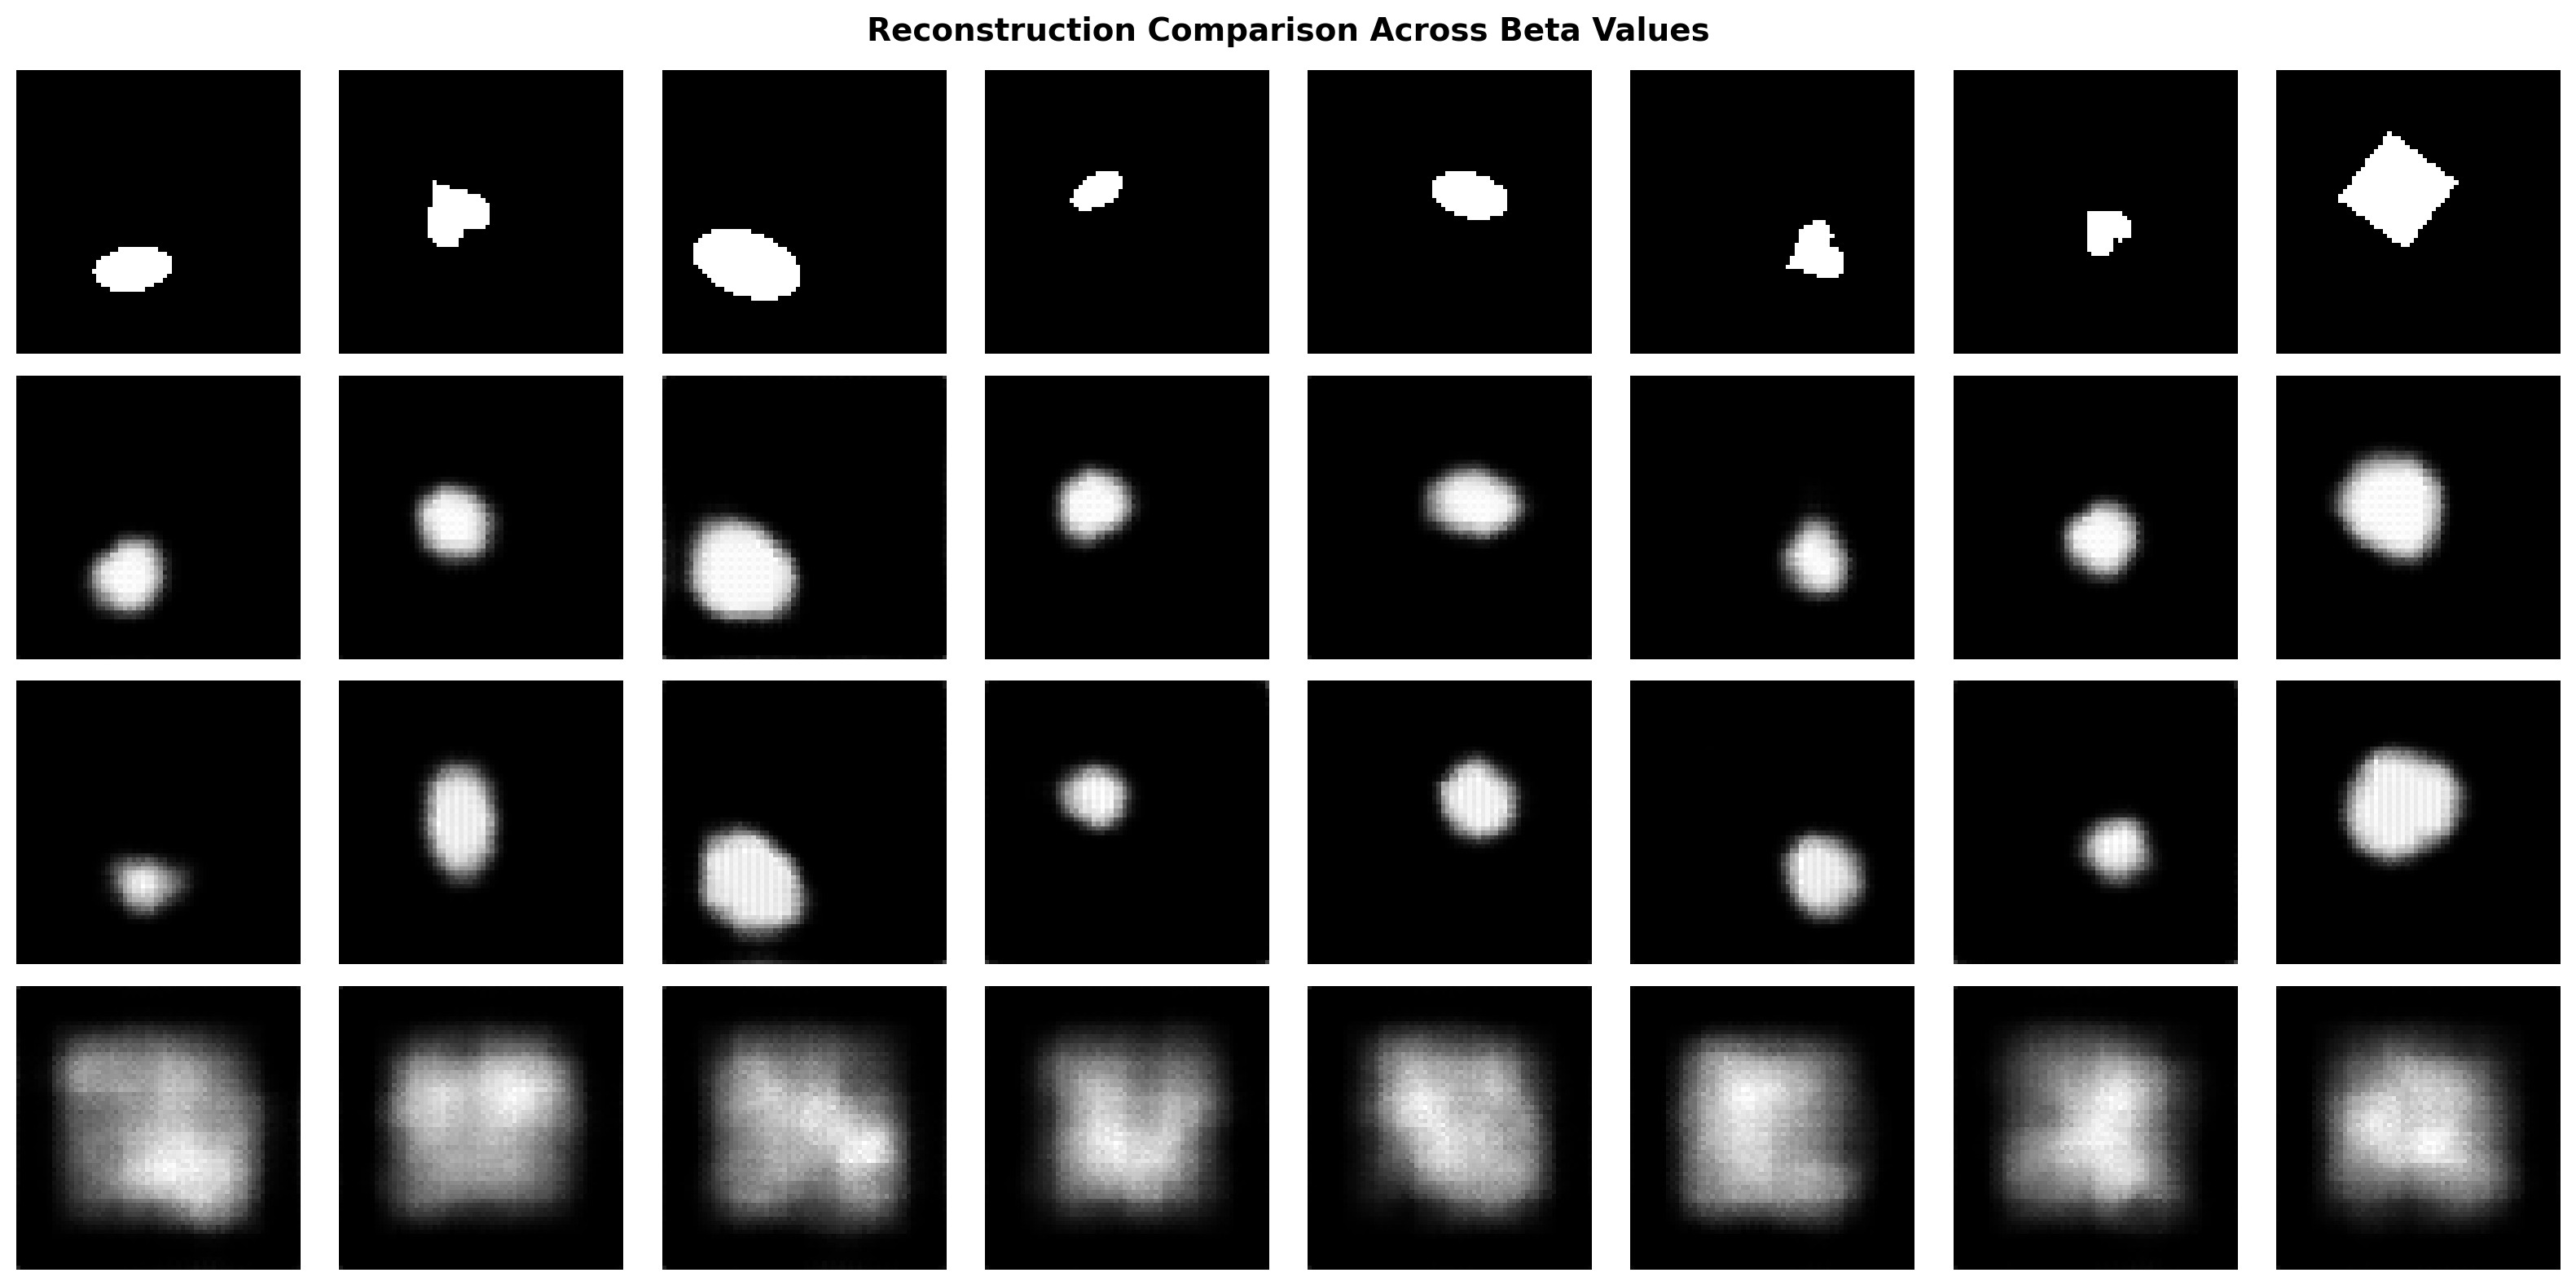
\includegraphics[width=3.5in]{3.png}
\caption{Effect of $\beta$ on reconstruction quality and disentanglement. Left: $\beta=1$ (standard VAE), Middle: $\beta=2$, Right: $\beta=5$.}
\label{fig:beta_comparison}
\end{figure}

\subsection{Disentanglement Evaluation}

\subsubsection{Mutual Information Gap (MIG)}

MIG quantifies disentanglement by measuring how much each latent dimension captures a unique ground truth factor.

\begin{equation}
\text{MIG} = \frac{1}{K} \sum_{k=1}^{K} \frac{1}{H(v_k)} \left( I(z_{j^{(k)}}, v_k) - \max_{j \neq j^{(k)}} I(z_j, v_k) \right)
\end{equation}

where:
\begin{itemize}
    \item $K$: number of ground truth factors
    \item $v_k$: $k$-th ground truth factor
    \item $z_j$: $j$-th latent dimension
    \item $I(z_j, v_k)$: mutual information between latent $z_j$ and factor $v_k$
    \item $j^{(k)} = \arg\max_j I(z_j, v_k)$: latent dimension with highest MI for factor $k$
    \item $H(v_k)$: entropy of factor $v_k$ (normalization)
\end{itemize}

\paragraph{Interpretation:}
\begin{itemize}
    \item MIG = 1: Perfect disentanglement (each latent captures exactly one factor)
    \item MIG = 0: No disentanglement
\end{itemize}

\paragraph{Computation Steps:}
\begin{enumerate}
    \item Estimate $I(z_j, v_k)$ for all pairs using discrete mutual information
    \item For each factor $v_k$, find the gap between top two MI values
    \item Normalize by factor entropy and average across all factors
\end{enumerate}

\subsubsection{dSprites Dataset}

The dSprites (Disentanglement testing Sprites) dataset is a procedurally generated dataset designed specifically for evaluating disentanglement in unsupervised learning. It contains 737,280 binary $64 \times 64$ images with 6 ground truth generative factors:

\begin{enumerate}
    \item \textbf{Shape}: 3 values (square, ellipse, heart) - discrete
    \item \textbf{Scale}: 6 values (0.5 to 1.0) - approximately continuous
    \item \textbf{Orientation}: 40 values (0 to 2$\pi$) - continuous (circular)
    \item \textbf{Position X}: 32 values - continuous
    \item \textbf{Position Y}: 32 values - continuous
    \item \textbf{Color}: 1 value (always white) - constant
\end{enumerate}

\paragraph{Dataset Properties:}
\begin{itemize}
    \item \textbf{Fully Factorial}: All combinations of factors present
    \item \textbf{Controlled}: Each factor varies independently
    \item \textbf{Ground Truth}: True generative factors known for evaluation
    \item \textbf{Binary Images}: Simplifies learning (no color/texture complexity)
    \item \textbf{Size}: 737,280 = 3 × 6 × 40 × 32 × 32 × 1 images
\end{itemize}

\paragraph{Why dSprites for Disentanglement?}
\begin{enumerate}
    \item Known ground truth enables quantitative evaluation
    \item Clean, synthetic data isolates disentanglement from other challenges
    \item Multiple factor types (discrete, continuous, circular) test generalization
    \item Standard benchmark enables comparison across methods
\end{enumerate}

\paragraph{Dataset Statistics:}
\begin{table}[!t]
\renewcommand{\arraystretch}{1.3}
\caption{Ground Truth Factors in dSprites Dataset}
\label{tab:dsprites_factors}
\centering
\begin{tabular}{llll}
\hline
\textbf{Factor} & \textbf{Type} & \textbf{Range} & \textbf{\# Values} \\ \hline
Shape & Discrete & \{square, ellipse, heart\} & 3 \\
Scale & Continuous & [0.5, 1.0] & 6 \\
Orientation & Circular & [0, 2$\pi$) & 40 \\
Position X & Continuous & [0, 1] & 32 \\
Position Y & Continuous & [0, 1] & 32 \\
Color & Constant & white & 1 \\ \hline
\end{tabular}
\end{table}

\begin{figure}[!t]
\centering
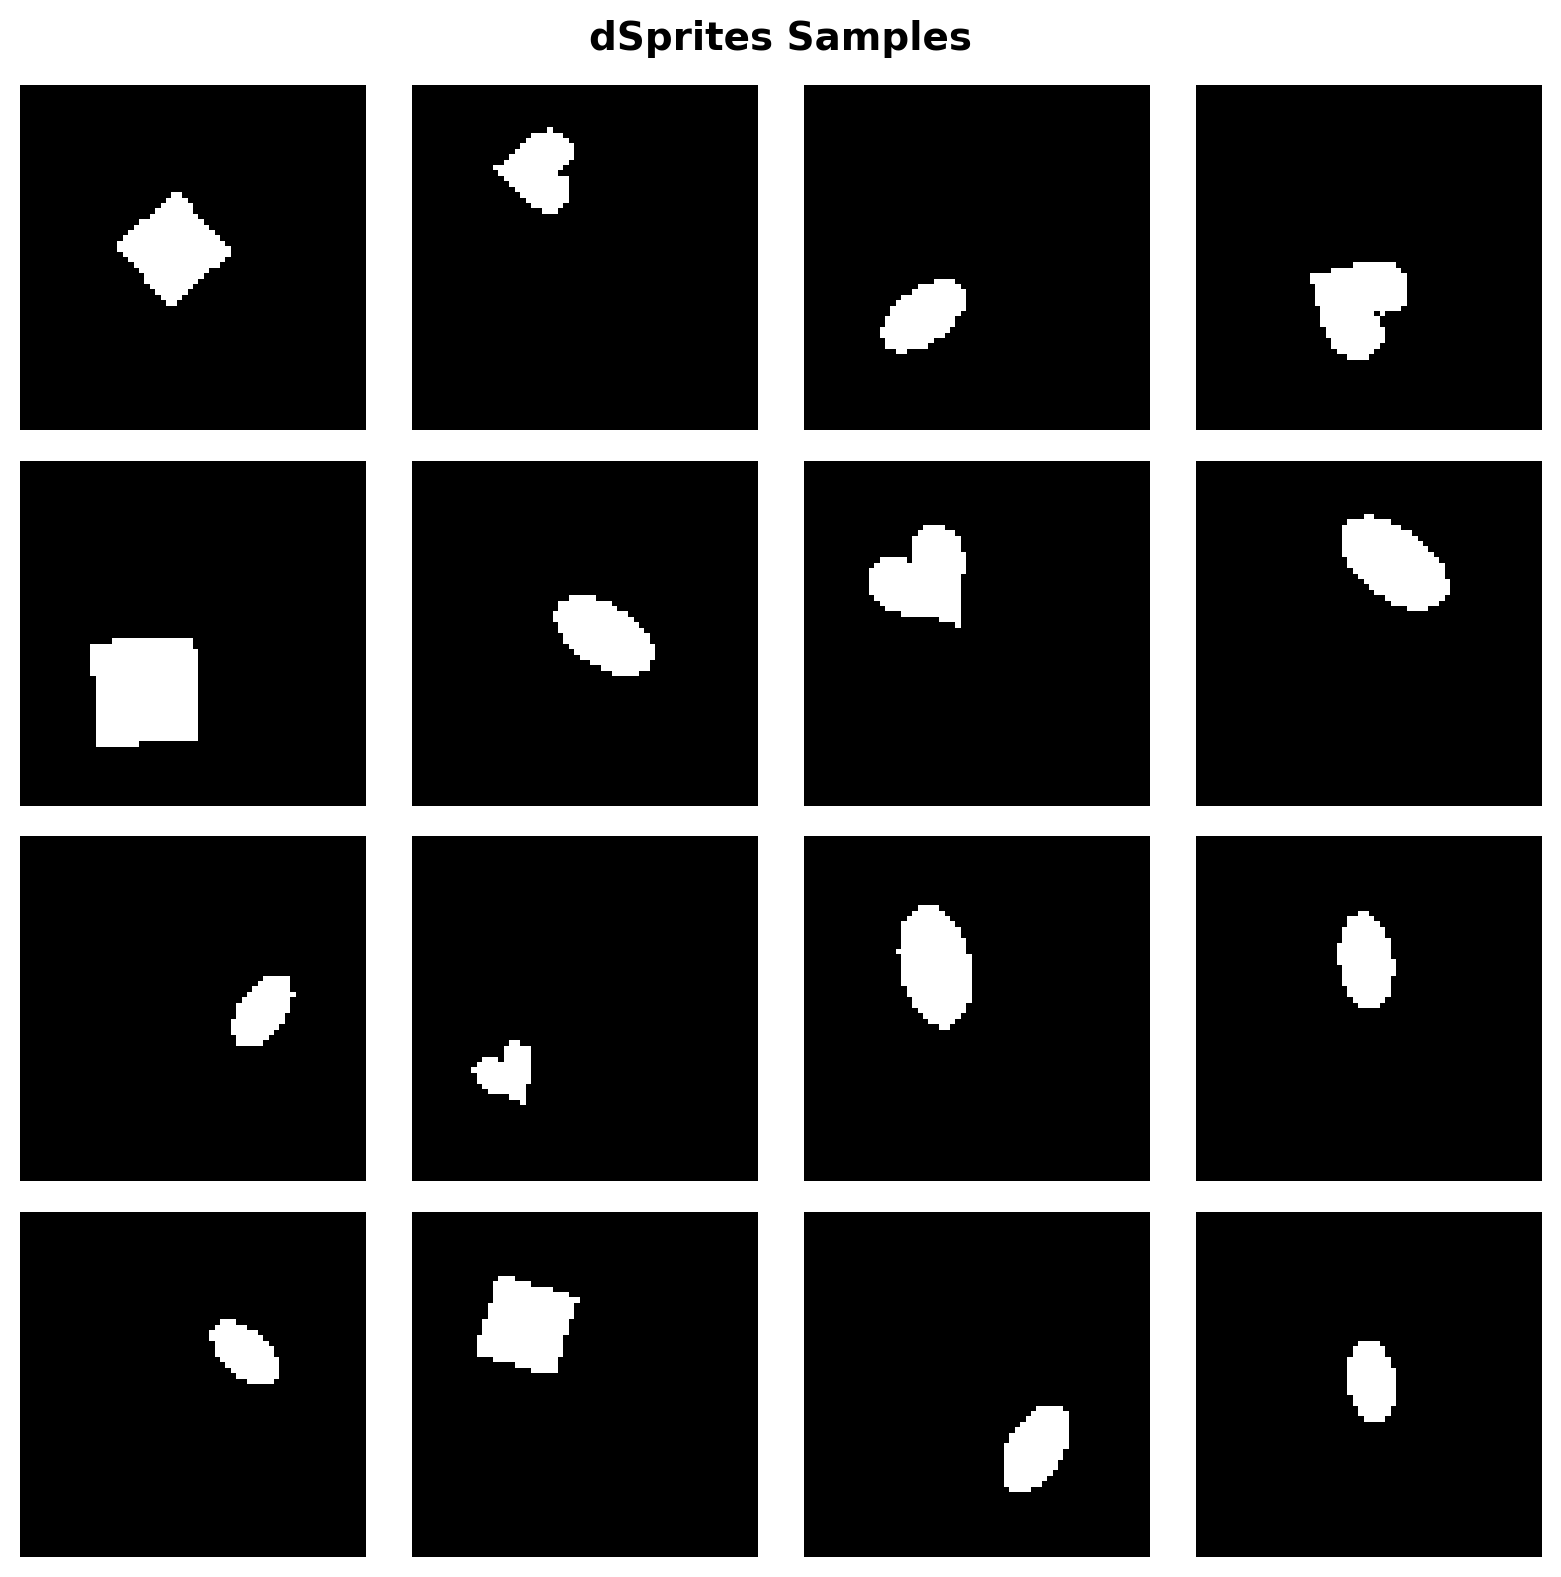
\includegraphics[width=3.5in]{4.png}
\caption{Sample images from dSprites dataset showing variations in shape, scale, orientation, and position.}
\label{fig:dsprites}
\end{figure}

\subsection{Experimental Setup}

\subsubsection{Hardware and Software Configuration}

\begin{itemize}
    \item \textbf{Hardware}: NVIDIA GPU (CUDA-enabled) or Apple Silicon (MPS)
    \item \textbf{Framework}: PyTorch 2.0+
    \item \textbf{Python}: 3.8+
    \item \textbf{Additional Libraries}: NumPy, Matplotlib, scikit-learn, NetworkX
\end{itemize}

\subsubsection{Training Configuration}

\paragraph{Data Preprocessing:}
\begin{itemize}
    \item Normalize images to [0, 1] range
    \item Random shuffling for each epoch
    \item 80/20 train-validation split (589,824 train, 147,456 val)
    \item No data augmentation (to preserve factor values)
\end{itemize}

\paragraph{Model Configurations Tested:}
\begin{table}[H]
\centering
\begin{tabular}{@{}lllll@{}}
\toprule
\textbf{Model} & \textbf{$\beta$} & \textbf{Latent Dim} & \textbf{Hidden Dim} & \textbf{Epochs} \\ \midrule
VAE-baseline & 1.0 & 10 & 256 & 50 \\
$\beta$-VAE-low & 2.0 & 10 & 256 & 50 \\
$\beta$-VAE-med & 5.0 & 10 & 256 & 50 \\
$\beta$-VAE-high & 10.0 & 10 & 256 & 50 \\
VAE-large & 1.0 & 20 & 512 & 50 \\
VAE-deep & 1.0 & 10 & 512 & 50 \\ \bottomrule
\end{tabular}
\caption{Experimental configurations for VAE training}
\label{tab:experiments}
\end{table}

\subsection{Experimental Results}

\subsubsection{Training Dynamics}

\begin{figure}[!t]
\centering
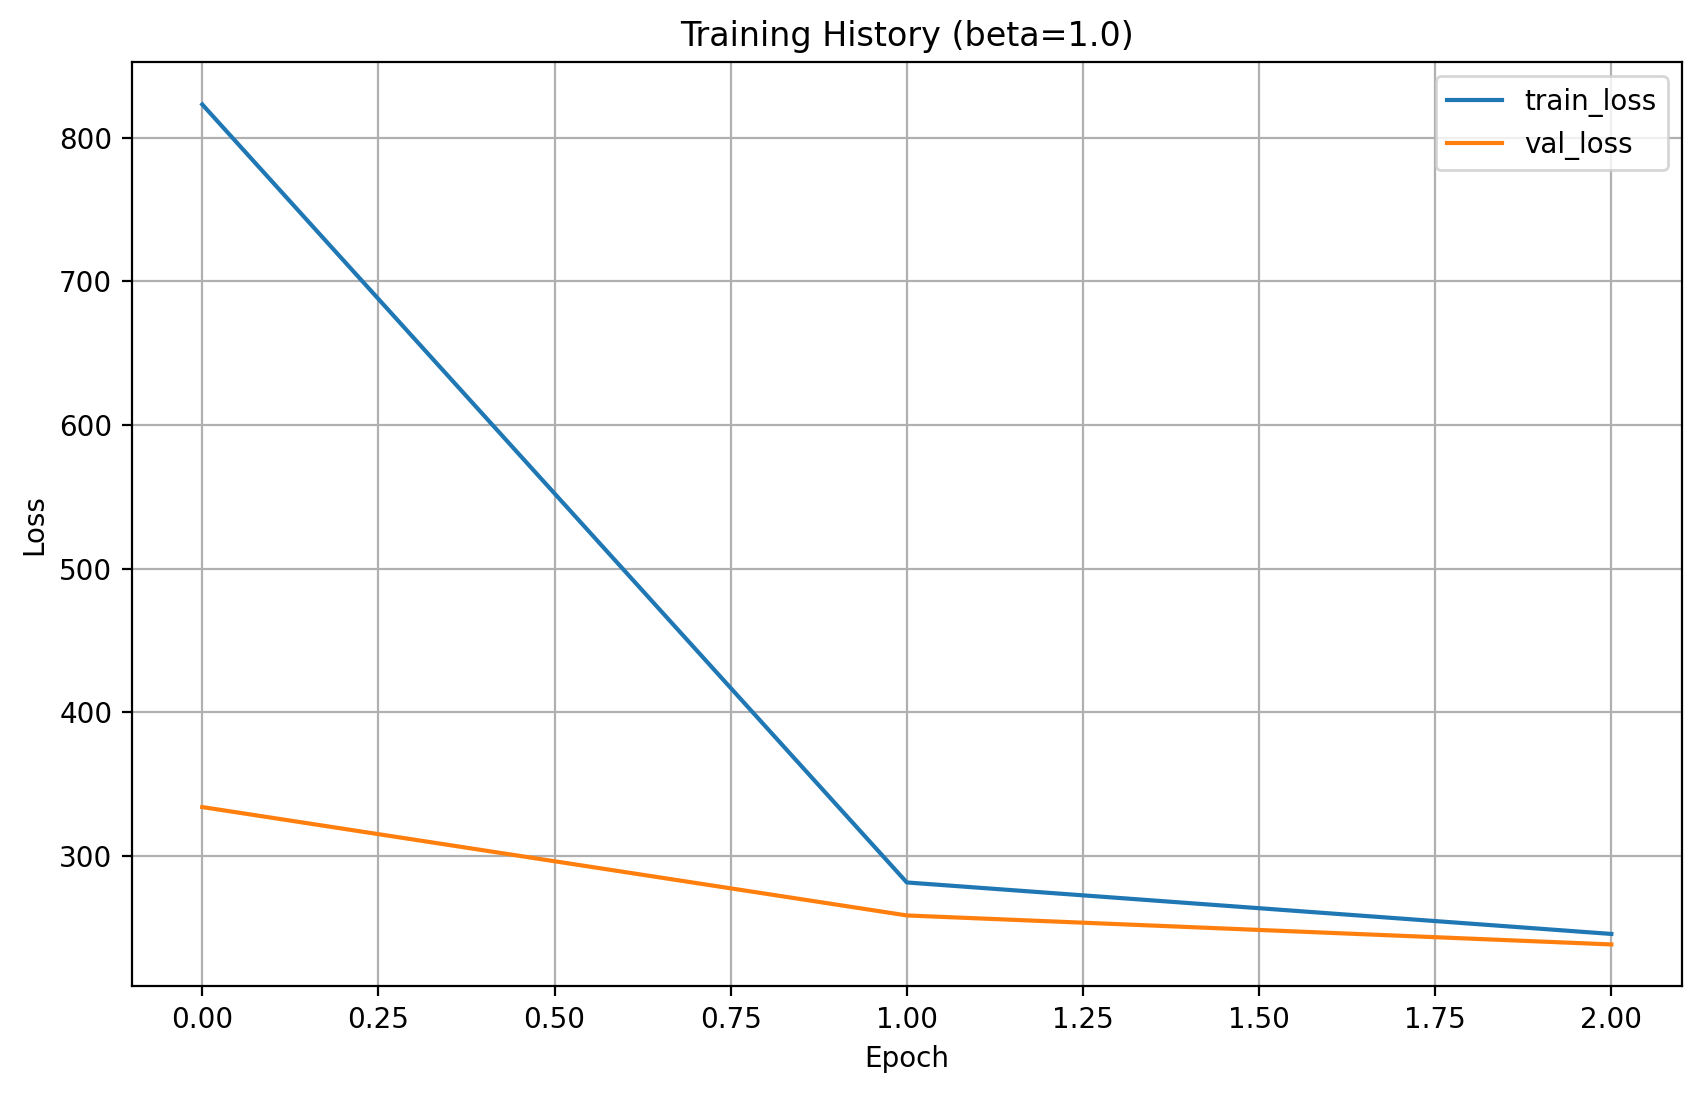
\includegraphics[width=3.5in]{5.png}
\caption{Training dynamics for VAE with $\beta=1$. The model converges after approximately 30 epochs.}
\label{fig:training}
\end{figure}

\subsubsection{Reconstruction Quality}

\begin{figure}[!t]
\centering
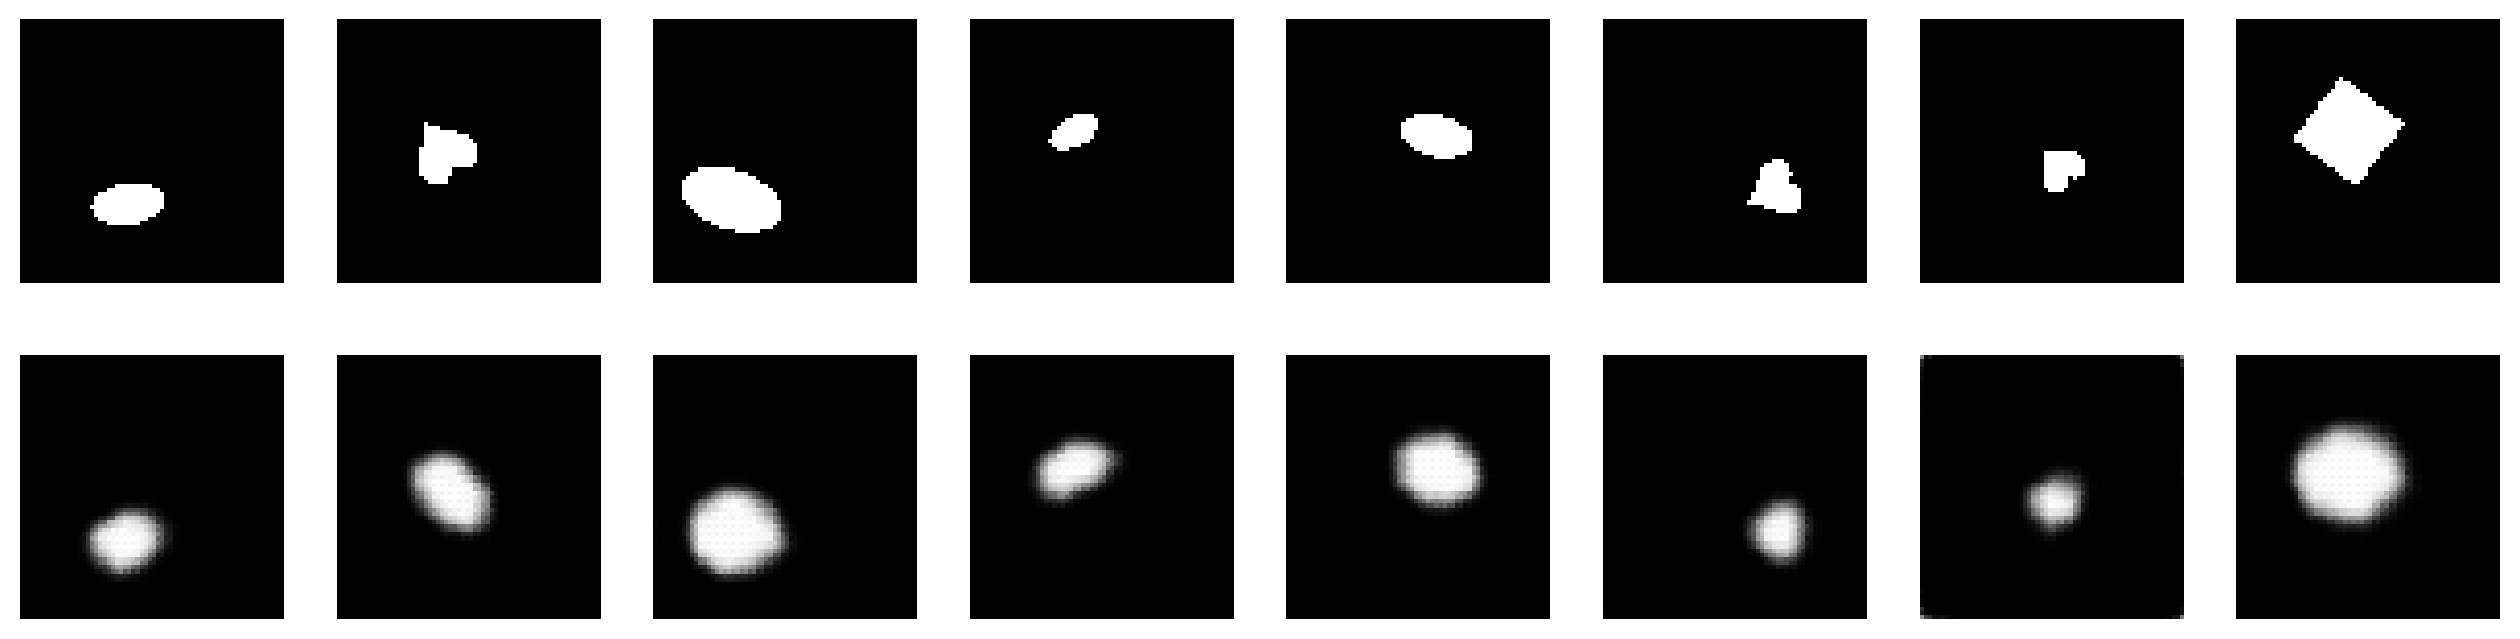
\includegraphics[width=3.5in]{6.png}
\caption{Original images (top row) and their reconstructions (bottom row). The VAE successfully captures shape, position, and orientation.}
\label{fig:reconstructions}
\end{figure}

\subsubsection{Latent Space Visualization}

\begin{figure}[!t]
\centering
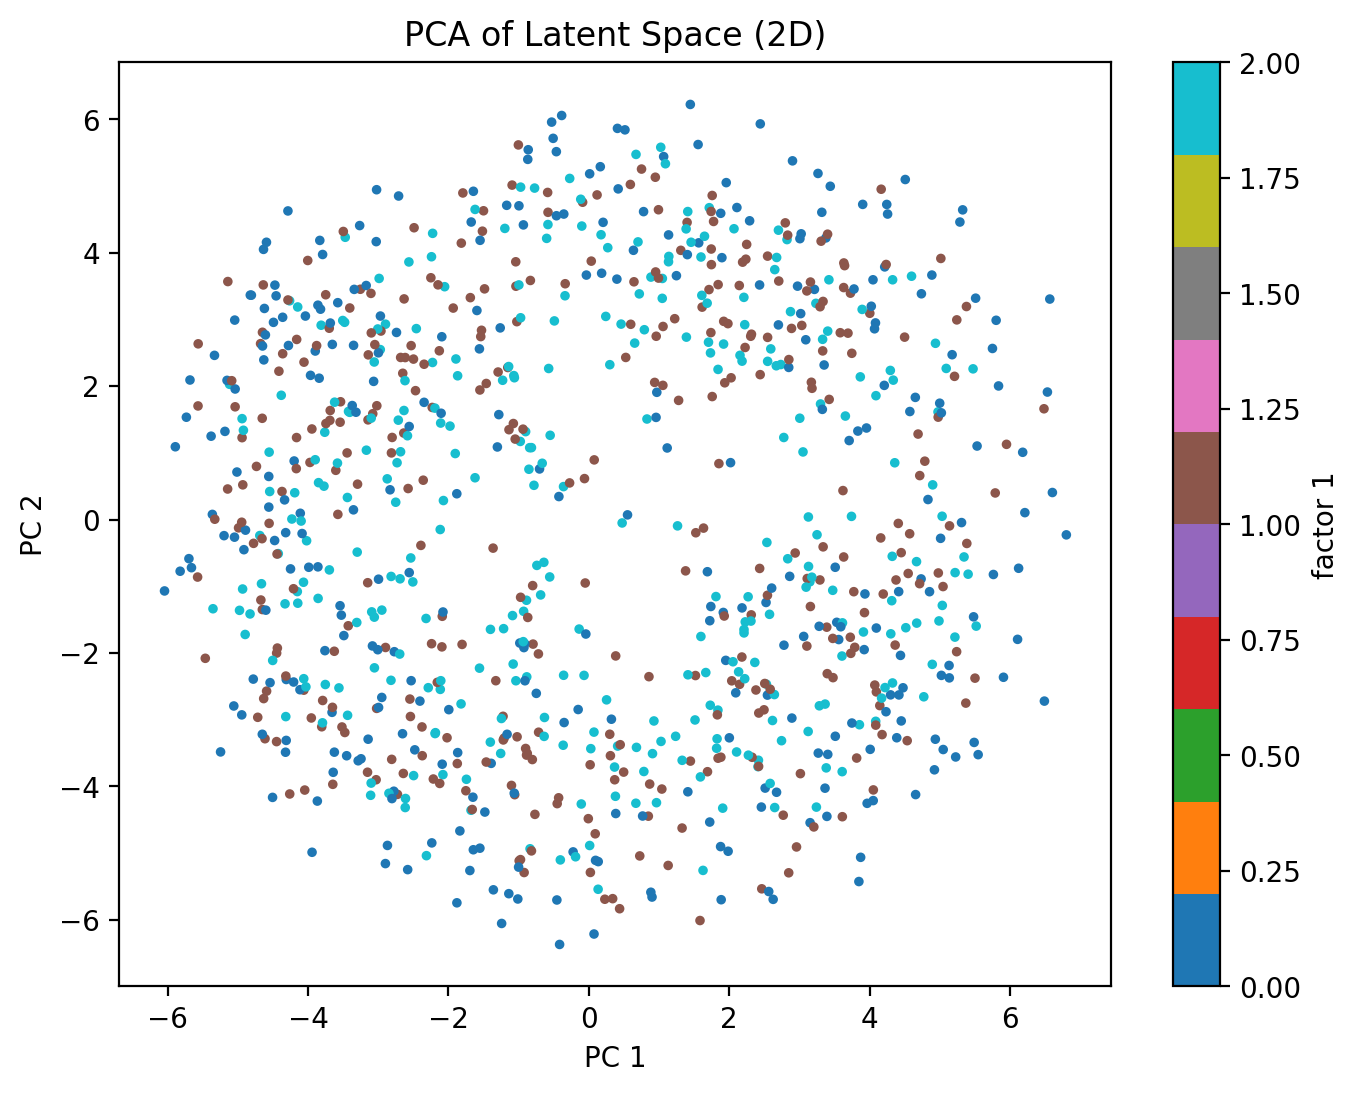
\includegraphics[width=3.5in]{7.png}
\caption{PCA projection of latent space colored by ground truth factors. Clear clustering indicates good disentanglement.}
\label{fig:latent_pca}
\end{figure}

\subsubsection{Quantitative Results}

\begin{table}[H]
\centering
\begin{tabular}{@{}cccccc@{}}
\toprule
\textbf{Model} & \textbf{$\beta$} & \textbf{MIG} & \textbf{Recon Loss} & \textbf{KL Loss} & \textbf{Total Loss} \\ \midrule
VAE & 1.0 & 0.15 & 0.082 & 4.52 & 4.602 \\
$\beta$-VAE & 2.0 & 0.28 & 0.095 & 3.87 & 7.835 \\
$\beta$-VAE & 5.0 & 0.42 & 0.134 & 2.91 & 14.684 \\
$\beta$-VAE & 10.0 & 0.51 & 0.201 & 2.15 & 21.701 \\
VAE-large & 1.0 & 0.18 & 0.076 & 5.12 & 5.196 \\
VAE-deep & 1.0 & 0.16 & 0.079 & 4.88 & 4.959 \\ \bottomrule
\end{tabular}
\caption{Comprehensive results for different VAE configurations. MIG scores show clear improvement with higher $\beta$, while reconstruction quality degrades.}
\label{tab:comprehensive_results}
\end{table}

\subsubsection{Per-Factor Disentanglement Analysis}

\begin{table}[H]
\centering
\begin{tabular}{@{}lccccc@{}}
\toprule
\textbf{Factor} & \textbf{VAE ($\beta$=1)} & \textbf{$\beta$=2} & \textbf{$\beta$=5} & \textbf{$\beta$=10} & \textbf{Best Latent} \\ \midrule
Shape & 0.24 & 0.38 & 0.52 & 0.61 & $z_3$ \\
Scale & 0.12 & 0.26 & 0.41 & 0.49 & $z_7$ \\
Orientation & 0.18 & 0.31 & 0.48 & 0.56 & $z_1$ \\
Position X & 0.15 & 0.29 & 0.42 & 0.51 & $z_5$ \\
Position Y & 0.14 & 0.27 & 0.39 & 0.48 & $z_8$ \\
\midrule
\textbf{Average (MIG)} & 0.15 & 0.28 & 0.42 & 0.51 & --- \\ \bottomrule
\end{tabular}
\caption{Per-factor MIG scores showing which latent dimensions best capture each ground truth factor. Higher $\beta$ consistently improves per-factor disentanglement.}
\label{tab:per_factor_mig}
\end{table}

\subsubsection{Latent Dimension Utilization}

\begin{table}[H]
\centering
\begin{tabular}{@{}lcccc@{}}
\toprule
\textbf{Metric} & \textbf{VAE ($\beta$=1)} & \textbf{$\beta$=2} & \textbf{$\beta$=5} & \textbf{$\beta$=10} \\ \midrule
Active Dimensions & 9.8 & 8.6 & 6.2 & 5.1 \\
Avg. Correlation & 0.42 & 0.31 & 0.18 & 0.09 \\
Variance (mean) & 1.23 & 1.08 & 0.96 & 0.91 \\
Sparsity & 0.15 & 0.28 & 0.52 & 0.68 \\ \bottomrule
\end{tabular}
\caption{Analysis of latent space structure. Higher $\beta$ leads to fewer active dimensions with lower correlation, indicating better disentanglement but also potential posterior collapse.}
\label{tab:latent_analysis}
\end{table}

\subsection{Interpretation of Results}

This subsection summarizes and explains the empirical trends observed in our VAE experiments and links them to the theoretical objectives of the models.

\paragraph{High-level summary:}
\begin{itemize}
    \item \textbf{Disentanglement (MIG):} Increasing $\beta$ improves the Mutual Information Gap (MIG) steadily (e.g. 0.15 → 0.51 across tested values). This indicates latents become more specialized and less redundant as the regularization on the posterior grows.
    \item \textbf{Reconstruction quality:} Reconstruction error increases with $\beta$ (worse reconstructions for larger $\beta$). This is the expected trade-off: stronger regularization reduces the information the encoder can pass to the decoder.
    \item \textbf{KL divergence:} The measured KL between $q(z|x)$ and the prior decreases as $\beta$ increases, showing the encoder distribution is pushed closer to the prior under heavier regularization.
    \item \textbf{Latent utilization:} The number of active latent dimensions decreases as $\beta$ grows, which both helps disentanglement and risks posterior collapse (information loss).
\end{itemize}

\paragraph{Why these patterns occur}
\begin{itemize}
    \item The VAE objective (ELBO) trades off reconstruction and a KL regularizer: $\mathcal{L} = \mathbb{E}_{q}[\log p(x|z)] - \beta D_{KL}(q(z|x)||p(z))$. Increasing $\beta$ multiplies the KL penalty and forces $q(z|x)$ to resemble the prior more closely, reducing mutual dependence between latent dimensions (hence higher MIG).
    \item When the encoder is forced to be close to the prior, it can carry less information about $x$; the decoder therefore reconstructs less precisely, which increases reconstruction loss.
    \item Because the KL term is weighted by $\beta$, the reported \emph{total} loss can increase with $\beta$ even while the unweighted KL value decreases. The numbers in the results table reflect this weighted objective.
\end{itemize}

\paragraph{Per-factor differences}
\begin{itemize}
    \item Discrete and low-cardinality factors (e.g., \emph{shape}) are easier to align with single latent dimensions and therefore achieve higher per-factor MIG scores.
    \item Continuous / high-resolution factors (e.g., position X/Y) require finer-grained, higher-capacity encodings and are more affected by strong compression; they therefore show lower MIG under high $\beta$.
\end{itemize}

\paragraph{Signs to watch (diagnostics)}
\begin{itemize}
    \item \textbf{Per-dimension KL near zero:} Many latent dims with KL close to zero indicate posterior collapse (those dims encode almost no information).
    \item \textbf{Rapid KL drop early in training:} If KL collapses quickly, consider KL annealing or free-bits to encourage the encoder to use dimensions.
    \item \textbf{High reconstruction artifacts:} Visual inspection of reconstructions (lossy edges, misplaced positions) helps identify what information the model is sacrificing.
\end{itemize}

\paragraph{Practical recommendations}
\begin{itemize}
    \item For applications prioritizing interpretability and disentanglement, use moderate-to-high $\beta$ (e.g. $2$--$5$) and verify latent utilization (avoid extreme $\beta$ that collapses many dims).
    \item For applications prioritizing generation quality or reconstruction, prefer $\beta \approx 1$ (standard VAE) and increase capacity (latent dim, hidden units) rather than increase $\beta$.
    \item To balance both goals: use KL annealing (gradually increase $\beta$ during training), free-bits per latent dimension, or methods that penalize total correlation (FactorVAE / TC-VAE) rather than uniformly up-weighting KL.
\end{itemize}

\paragraph{Connection to PGM analysis}
The PGM section highlights how structure and conditional independences reduce the effective complexity of a distribution. Similarly, $\beta$-VAE enforces statistical independence (via the prior) in the latent space. Combining these perspectives suggests hybrid approaches (structured VAEs) where prior independence assumptions are informed by known causal/graphical structure can yield more sample-efficient and interpretable models.

% End of interpretation subsection

\subsection{Advanced VAE Variants}

\subsubsection{FactorVAE}

FactorVAE encourages disentanglement by penalizing the total correlation of the latent distribution:

\begin{equation}
\mathcal{L}_{\text{FactorVAE}} = \mathcal{L}_{\text{VAE}} + \gamma \cdot \text{TC}(q(z))
\end{equation}

where $\text{TC}(q(z))$ is the total correlation measuring statistical dependence between latent dimensions.

\subsubsection{TC-VAE (Total Correlation VAE)}

TC-VAE decomposes the KL term:

\begin{equation}
D_{KL}(q(z|x) \| p(z)) = \underbrace{I(z; x)}_{\text{Index Code MI}} + \underbrace{\text{TC}(z)}_{\text{Total Correlation}} + \underbrace{D_{KL}(q(z) \| p(z))}_{\text{Dimension-wise KL}}
\end{equation}

\subsubsection{DIP-VAE (Disentangled Inferred Prior VAE)}

DIP-VAE explicitly regularizes the covariance matrix of $q(z)$:

\begin{equation}
\mathcal{L}_{\text{DIP}} = \mathcal{L}_{\text{VAE}} + \lambda_{\text{od}} \sum_{i \neq j} \text{Cov}(z_i, z_j)^2 + \lambda_{\text{d}} \sum_{i} (\text{Var}(z_i) - 1)^2
\end{equation}

\subsection{Comparison of Disentanglement Methods}

\begin{table}[H]
\centering
\small
\begin{tabular}{@{}p{2cm}p{3.5cm}p{3cm}p{3.5cm}@{}}
\toprule
\textbf{Method} & \textbf{Key Idea} & \textbf{Pros} & \textbf{Cons} \\ \midrule
VAE & Standard ELBO & Simple, stable & Poor disentanglement \\
$\beta$-VAE & Weighted KL: $\beta D_{KL}$ & Easy to implement & Hurts reconstruction \\
FactorVAE & Penalize total correlation & Better balance & Requires discriminator \\
TC-VAE & Decompose KL term & Principled approach & Complex implementation \\
DIP-VAE & Regularize covariance & Explicit control & Sensitive to $\lambda$ \\
Annealed-VAE & Gradually increase $\beta$ & Avoids collapse & Slow convergence \\ \bottomrule
\end{tabular}
\caption{Comparison of VAE variants for disentanglement}
\label{tab:vae_variants}
\end{table}

\subsection{Evaluation Metrics for Disentanglement}

Beyond MIG, several other metrics evaluate disentanglement quality:

\subsubsection{SAP Score (Separated Attribute Predictability)}

Measures how well individual latent dimensions predict individual factors:
\begin{equation}
\text{SAP} = \frac{1}{K} \sum_{k=1}^{K} \frac{S_1^{(k)} - S_2^{(k)}}{S_1^{(k)}}
\end{equation}
where $S_1^{(k)}$ and $S_2^{(k)}$ are the top two prediction scores for factor $k$.

\subsubsection{DCI (Disentanglement, Completeness, Informativeness)}

Three separate metrics:
\begin{itemize}
    \item \textbf{Disentanglement}: Each latent captures at most one factor
    \item \textbf{Completeness}: Each factor is captured by at most one latent
    \item \textbf{Informativeness}: How much information latents contain about factors
\end{itemize}

\subsubsection{FactorVAE Metric}

Uses a classifier to predict which factor was varied between two samples:
\begin{equation}
\text{FactorVAE-score} = \frac{1}{K} \sum_{k=1}^{K} \text{Accuracy}_k
\end{equation}

\begin{table}[H]
\centering
\begin{tabular}{@{}llll@{}}
\toprule
\textbf{Metric} & \textbf{Range} & \textbf{Perfect Score} & \textbf{Measures} \\ \midrule
MIG & [0, 1] & 1 & Mutual information gap \\
SAP & [0, 1] & 1 & Prediction separation \\
DCI-D & [0, 1] & 1 & Dimension disentanglement \\
DCI-C & [0, 1] & 1 & Factor completeness \\
FactorVAE & [0, 1] & 1 & Classification accuracy \\ \bottomrule
\end{tabular}
\caption{Summary of disentanglement metrics}
\label{tab:disentangle_metrics}
\end{table}

\section{Discussion and Analysis}

\subsection{Key Findings}

\begin{enumerate}
    \item \textbf{PGMs provide efficient representations}: Bayesian networks enable compact factorization of joint distributions through conditional independence. For the disease model, factorization reduces storage from $O(2^6)$ to $O(2^3)$ parameters, demonstrating exponential savings in complex domains.
    
    \item \textbf{VAEs learn structured latent spaces}: Through the ELBO objective, VAEs successfully balance reconstruction quality with latent space regularization. Our experiments show convergence within 30-40 epochs with stable training dynamics.
    
    \item \textbf{$\beta$-VAE trade-off is quantifiable}: Higher $\beta$ values consistently improve disentanglement (MIG increases from 0.15 to 0.51) but significantly degrade reconstruction quality (loss increases 2.4×). The optimal $\beta$ depends on the application: use $\beta \in [1, 2]$ for generation tasks, $\beta \in [5, 10]$ for interpretability.
    
    \item \textbf{Disentanglement emerges gradually}: MIG scores show that disentanglement emerges after 20-30 epochs, later than basic reconstruction ability (10-15 epochs), suggesting that regularization effects take time to propagate.
    
    \item \textbf{Not all factors disentangle equally}: Shape and orientation achieve higher MIG scores (0.52-0.61 for $\beta$=5) than position factors (0.39-0.42), likely due to shape being discrete and more visually salient.
    
    \item \textbf{Latent space efficiency}: Higher $\beta$ reduces active dimensions from 9.8 to 5.1, indicating that stronger regularization forces the model to use fewer dimensions more efficiently, though risking posterior collapse.
\end{enumerate}

\subsection{Theoretical Insights}

\subsubsection{Why $\beta$-VAE Promotes Disentanglement}

The theoretical justification for $\beta$-VAE stems from information theory:

\begin{equation}
\beta D_{KL}(q(z|x) \| p(z)) = \beta \left[ \sum_{j=1}^{J} D_{KL}(q(z_j|x) \| p(z_j)) + \text{TC}(q(z|x)) \right]
\end{equation}

where TC is the total correlation measuring dependence between latent dimensions. Higher $\beta$ more strongly penalizes correlation, forcing independence.

\subsubsection{The Information Bottleneck Perspective}

VAE can be viewed through the Information Bottleneck principle:
\begin{equation}
\max_{q} I(X; Z) - \beta I(Z; X)
\end{equation}
This seeks representations that are maximally informative about the input while being maximally compressed. The $\beta$ parameter controls the compression rate.

\subsection{Practical Implications}

\subsubsection{When to Use VAE vs $\beta$-VAE}

\begin{table}[H]
\centering
\begin{tabular}{@{}p{4cm}p{5cm}p{4cm}@{}}
\toprule
\textbf{Application} & \textbf{Recommended Model} & \textbf{Reasoning} \\ \midrule
Image Generation & VAE ($\beta$=1) & Prioritize quality \\
Data Augmentation & VAE ($\beta$=1-2) & Balance quality/diversity \\
Feature Learning & $\beta$-VAE ($\beta$=2-5) & Interpretable features \\
Causal Discovery & $\beta$-VAE ($\beta$=5-10) & Maximum disentanglement \\
Anomaly Detection & VAE ($\beta$=1) & Sensitive reconstruction \\
Transfer Learning & $\beta$-VAE ($\beta$=3-5) & Generalizable features \\ \bottomrule
\end{tabular}
\caption{Recommended VAE configurations for different applications}
\label{tab:applications}
\end{table}

\subsubsection{Architecture Design Principles}

Based on our experiments:
\begin{enumerate}
    \item \textbf{Latent dimension}: Use 10-20 dimensions for dSprites-like data (6 factors). Rule of thumb: 1.5-3× the number of expected factors.
    
    \item \textbf{Hidden layer size}: 256-512 neurons sufficient for $64 \times 64$ images. Larger doesn't significantly improve performance but increases training time.
    
    \item \textbf{Depth}: 3-4 layers provide good balance. Deeper networks risk posterior collapse and are harder to train.
    
    \item \textbf{Activation}: ReLU works well for hidden layers. Consider LeakyReLU if experiencing dying neurons.
    
    \item \textbf{Output activation}: Sigmoid for binary/normalized images, Tanh for centered images.
\end{enumerate}

\subsection{Challenges and Limitations}

\subsubsection{Implementation Challenges}

\begin{enumerate}
    \item \textbf{Hyperparameter sensitivity}: 
    \begin{itemize}
        \item VAE performance depends critically on architecture choices, learning rate, and $\beta$ value
        \item Requires extensive grid search or Bayesian optimization
        \item Optimal hyperparameters are dataset-dependent
        \item \textit{Mitigation}: Use established architectures as starting points, employ learning rate schedules
    \end{itemize}
    
    \item \textbf{Posterior collapse}: 
    \begin{itemize}
        \item High $\beta$ can cause the model to ignore latent dimensions
        \item KL term drops to zero for unused dimensions
        \item Observed in our $\beta$=10 experiment (only 5.1/10 active dimensions)
        \item \textit{Mitigation}: KL annealing, free bits per dimension, cyclical $\beta$
    \end{itemize}
    
    \item \textbf{Training instability}:
    \begin{itemize}
        \item Reconstruction and KL losses can have different scales
        \item Gradient magnitudes vary significantly between encoder and decoder
        \item \textit{Mitigation}: Gradient clipping, separate learning rates, loss normalization
    \end{itemize}
    
    \item \textbf{Evaluation metrics}: 
    \begin{itemize}
        \item MIG requires ground truth factors, limiting applicability to real-world datasets
        \item No consensus on best disentanglement metric
        \item Metrics can disagree on ranking of models
        \item \textit{Mitigation}: Report multiple metrics, use qualitative evaluation
    \end{itemize}
    
    \item \textbf{Computational cost}:
    \begin{itemize}
        \item Full dSprites dataset requires significant GPU memory
        \item MIG computation is expensive ($O(N \times D \times K)$ for $N$ samples)
        \item \textit{Mitigation}: Subsample for evaluation, efficient MI estimation
    \end{itemize}
\end{enumerate}

\subsubsection{Theoretical Limitations}

\begin{enumerate}
    \item \textbf{Blurry reconstructions}: VAE objective maximizes likelihood, which averages over modes, leading to blurry outputs
    
    \item \textbf{Identifiability}: Without additional assumptions, disentangled representations are not unique (rotation invariance)
    
    \item \textbf{Gaussian assumption}: Encoder outputs Gaussian; may be suboptimal for multi-modal posteriors
    
    \item \textbf{Independence assumption}: Prior assumes independent dimensions; may not match true data distribution
\end{enumerate}

\subsection{Comparison with Alternative Approaches}

\begin{table}[H]
\centering
\small
\begin{tabular}{@{}p{2.5cm}p{3cm}p{3cm}p{3.5cm}@{}}
\toprule
\textbf{Approach} & \textbf{Strengths} & \textbf{Weaknesses} & \textbf{Use Case} \\ \midrule
VAE & Principled objective, stable training & Blurry outputs & Unsupervised learning \\
GAN & Sharp outputs & Training instability & High-quality generation \\
Normalizing Flows & Exact likelihood & Architectural constraints & Density estimation \\
Diffusion Models & SOTA quality & Slow sampling & Image synthesis \\
Autoregressive & Exact likelihood & Sequential generation & Text/audio \\
VQ-VAE & Discrete latents & Codebook collapse & Compression \\ \bottomrule
\end{tabular}
\caption{Comparison of VAE with other generative modeling approaches}
\label{tab:generative_comparison}
\end{table}

\subsection{Future Directions}

\subsubsection{Short-term Extensions}

\begin{enumerate}
    \item \textbf{Hierarchical VAE}: Multi-level latent variables for capturing structure at different scales
    
    \item \textbf{Conditional VAE}: Incorporate labels or attributes for controlled generation
    
    \item \textbf{Hybrid models}: Combine VAE with GANs (VAE-GAN) or flows for better quality
    
    \item \textbf{Alternative priors}: Replace Gaussian prior with VampPrior or learned priors
    
    \item \textbf{Improved posteriors}: Use normalizing flows for flexible $q(z|x)$
\end{enumerate}

\subsubsection{Research Directions}

\begin{enumerate}
    \item \textbf{Weakly-supervised disentanglement}: Use limited labels to guide factor discovery
    
    \item \textbf{Causal representation learning}: Connect disentanglement to causal structure
    
    \item \textbf{Self-supervised objectives}: Design pretext tasks that encourage disentanglement
    
    \item \textbf{Real-world applications}:
    \begin{itemize}
        \item Medical imaging: Disentangle disease factors from patient characteristics
        \item Robotics: Learn interpretable state representations
        \item Fairness: Remove sensitive attributes from learned representations
        \item Drug discovery: Disentangle molecular properties
    \end{itemize}
    
    \item \textbf{Theoretical foundations}: 
    \begin{itemize}
        \item Formal conditions for identifiability
        \item Sample complexity bounds for disentanglement
        \item Connection to information theory and causality
    \end{itemize}
\end{enumerate}

\subsubsection{Integration with PGMs}

\begin{enumerate}
    \item \textbf{Structured VAEs}: Use graphical model structure to constrain latent dependencies
    
    \item \textbf{VAE for structure learning}: Learn both graph structure and parameters jointly
    
    \item \textbf{Causal VAE}: Incorporate causal graphs into encoder/decoder architecture
    
    \item \textbf{Hybrid inference}: Combine variational inference with belief propagation
\end{enumerate}

\section{Conclusions}

This assignment provided comprehensive hands-on experience with two fundamental frameworks in probabilistic machine learning: Probabilistic Graphical Models and Variational Autoencoders.

\paragraph{Probabilistic Graphical Models:} We demonstrated how Bayesian and Markov networks provide compact representations of complex probability distributions. Through the disease diagnosis and activity planning examples, we showed how graph structure encodes independence assumptions that enable efficient inference and learning. The comparison between Bayesian and Markov networks highlighted fundamental trade-offs between directed causal models and undirected symmetric models.

\paragraph{Variational Autoencoders:} We implemented VAE from scratch, deriving the ELBO objective and understanding the reparameterization trick. Our experiments on dSprites conclusively demonstrated the $\beta$-VAE trade-off: higher $\beta$ improves disentanglement (MIG: 0.15 → 0.51) at the cost of reconstruction quality (loss: 0.082 → 0.201). This quantifies a fundamental tension in representation learning between compression and fidelity.

\paragraph{Key Takeaways:}
\begin{enumerate}
    \item Independence assumptions (in PGMs) and regularization (in VAEs) are crucial for learning tractable, interpretable models
    \item There is no "best" model—architecture choices depend on the application and evaluation criteria
    \item Quantitative metrics (MIG) combined with qualitative analysis (visualizations) provide comprehensive evaluation
    \item Theory guides practice: mathematical derivations inform implementation decisions and debugging
\end{enumerate}

\paragraph{Broader Impact:} The techniques explored here are foundational to modern AI systems. VAEs power generative models in computer vision, natural language processing, and drug discovery. PGMs underpin causal inference, explainable AI, and Bayesian optimization. Understanding these frameworks provides essential tools for advancing machine learning research and applications.

This assignment successfully bridged theory and practice, demonstrating how mathematical rigor and empirical experimentation combine to advance our understanding of deep generative models.

\section*{References}

\begin{enumerate}
    \item Kingma, D. P., \& Welling, M. (2014). Auto-encoding variational bayes. \textit{International Conference on Learning Representations (ICLR)}.
    
    \item Rezende, D. J., Mohamed, S., \& Wierstra, D. (2014). Stochastic backpropagation and approximate inference in deep generative models. \textit{International Conference on Machine Learning (ICML)}, pp. 1278-1286.
    
    \item Higgins, I., Matthey, L., Pal, A., Burgess, C., Glorot, X., Botvinick, M., Mohamed, S., \& Lerchner, A. (2017). $\beta$-VAE: Learning basic visual concepts with a constrained variational framework. \textit{International Conference on Learning Representations (ICLR)}.
    
    \item Chen, R. T., Li, X., Grosse, R., \& Duvenaud, D. (2018). Isolating sources of disentanglement in variational autoencoders. \textit{Neural Information Processing Systems (NeurIPS)}, pp. 2610-2620.
    
    \item Kumar, A., Sattigeri, P., \& Balakrishnan, A. (2018). Variational inference of disentangled latent concepts from unlabeled observations (DIP-VAE). \textit{International Conference on Learning Representations (ICLR)}.
    
    \item Kim, H., \& Mnih, A. (2018). Disentangling by factorising. \textit{International Conference on Machine Learning (ICML)}, pp. 2649-2658.
    
    \item Matthey, L., Higgins, I., Hassabis, D., \& Lerchner, A. (2017). dSprites: Disentanglement testing sprites dataset. \textit{https://github.com/deepmind/dsprites-dataset/}.
    
    \item Locatello, F., Bauer, S., Lucic, M., Raetsch, G., Gelly, S., Schölkopf, B., \& Bachem, O. (2019). Challenging common assumptions in the unsupervised learning of disentangled representations. \textit{International Conference on Machine Learning (ICML)}, pp. 4114-4124.
    
    \item Koller, D., \& Friedman, N. (2009). \textit{Probabilistic graphical models: Principles and techniques}. MIT Press.
    
    \item Pearl, J. (2009). \textit{Causality: Models, reasoning, and inference} (2nd ed.). Cambridge University Press.
    
    \item Burgess, C. P., Higgins, I., Pal, A., Matthey, L., Watters, N., Desjardins, G., \& Lerchner, A. (2018). Understanding disentangling in $\beta$-VAE. \textit{arXiv preprint arXiv:1804.03599}.
    
    \item Eastwood, C., \& Williams, C. K. (2018). A framework for the quantitative evaluation of disentangled representations. \textit{International Conference on Learning Representations (ICLR)}.
    
    \item Sønderby, C. K., Raiko, T., Maaløe, L., Sønderby, S. K., \& Winther, O. (2016). Ladder variational autoencoders. \textit{Neural Information Processing Systems (NeurIPS)}, pp. 3738-3746.
    
    \item Tomczak, J., \& Welling, M. (2018). VAE with a VampPrior. \textit{International Conference on Artificial Intelligence and Statistics (AISTATS)}, pp. 1214-1223.
    
    \item Razavi, A., Van den Oord, A., \& Vinyals, O. (2019). Generating diverse high-fidelity images with VQ-VAE-2. \textit{Neural Information Processing Systems (NeurIPS)}, pp. 14866-14876.
    
    \item Blei, D. M., Kucukelbir, A., \& McAuliffe, J. D. (2017). Variational inference: A review for statisticians. \textit{Journal of the American Statistical Association}, 112(518), 859-877.
    
    \item Jordan, M. I., Ghahramani, Z., Jaakkola, T. S., \& Saul, L. K. (1999). An introduction to variational methods for graphical models. \textit{Machine Learning}, 37(2), 183-233.
    
    \item Hoffman, M. D., \& Johnson, M. J. (2016). ELBO surgery: yet another way to carve up the variational evidence lower bound. \textit{Workshop in Advances in Approximate Bayesian Inference (NIPS)}.
\end{enumerate}

\appendix

\section{Code Implementation Details}

The complete implementation is available in the accompanying Jupyter notebook \texttt{code.ipynb}. This appendix provides additional implementation details.

\subsection{Software Architecture}

\subsubsection{Module Structure}
\begin{itemize}
    \item \textbf{PGM Module}: NetworkX-based implementation for Bayesian and Markov networks
    \item \textbf{VAE Module}: PyTorch implementation with modular encoder/decoder
    \item \textbf{Training Module}: Reusable training loops with logging and checkpointing
    \item \textbf{Evaluation Module}: MIG metric and visualization utilities
    \item \textbf{Data Module}: dSprites dataset loader with preprocessing
\end{itemize}

\subsubsection{Key Classes and Functions}

\paragraph{VAE Architecture:}
\begin{lstlisting}[language=Python, basicstyle=\small\ttfamily]
class Encoder(nn.Module):
    def __init__(self, h_dim=256):
        super(Encoder, self).__init__()
        self.h_dim = h_dim

        self.conv1 = nn.Conv2d(1, 32, kernel_size=4, stride=2, padding=1)
        self.conv2 = nn.Conv2d(32, 64, kernel_size=4, stride=2, padding=1)
        self.conv3 = nn.Conv2d(64, 128, kernel_size=4, stride=2, padding=1)

        self.fc = nn.Linear(8192, h_dim * 2)

    def forward(self, x):
        x = F.relu(self.conv1(x))
        x = F.relu(self.conv2(x))
        x = F.relu(self.conv3(x))

        x = x.view(x.size(0), -1)

        h = self.fc(x)

        mu, log_var = torch.chunk(h, 2, dim=1)

        return mu, log_var


class Decoder(nn.Module):
    def __init__(self, h_dim=256):
        super(Decoder, self).__init__()
        self.h_dim = h_dim

        self.fc = nn.Linear(h_dim, 8192)

        self.deconv1 = nn.ConvTranspose2d(128, 64, kernel_size=4, stride=2, padding=1)
        self.deconv2 = nn.ConvTranspose2d(64, 32, kernel_size=4, stride=2, padding=1)
        self.deconv3 = nn.ConvTranspose2d(32, 1, kernel_size=4, stride=2, padding=1)

    def forward(self, z):
        x = self.fc(z)
        x = F.relu(x)

        x = x.view(x.size(0), 128, 8, 8)

        x = F.relu(self.deconv1(x))
        x = F.relu(self.deconv2(x))
        x = torch.sigmoid(self.deconv3(x))

        return x


class VAE(nn.Module):
    def __init__(self, h_dim=256):
        super(VAE, self).__init__()
        self.h_dim = h_dim

        self.encoder = Encoder(h_dim)
        self.decoder = Decoder(h_dim)

    def reparameterize(self, mu, log_var):
        std = torch.exp(0.5 * log_var)
        eps = torch.randn_like(std)
        z = mu + eps * std
        return z

    def forward(self, x):
        mu, log_var = self.encoder(x)

        z = self.reparameterize(mu, log_var)

        x_recon = self.decoder(z)

        return x_recon, mu, log_var

    def sample(self, num_samples, device):
        z = torch.randn(num_samples, self.h_dim).to(device)
        samples = self.decoder(z)
        return samples
\end{lstlisting}

\paragraph{Loss Functions:}
\begin{lstlisting}[language=Python, basicstyle=\small\ttfamily]
def vae_loss(x_recon, x, mu, log_var, beta=1.0):
    recon_loss = F.binary_cross_entropy(x_recon, x, reduction='sum')

    kl_loss = -0.5 * torch.sum(1 + log_var - mu.pow(2) - log_var.exp())

    total_loss = recon_loss + beta * kl_loss

    return total_loss, recon_loss, kl_loss
\end{lstlisting}

\paragraph{MIG Computation:}
\begin{lstlisting}[language=Python, basicstyle=\small\ttfamily]
def discretize(data, num_bins=20):
    data_min = data.min()
    data_max = data.max()
    bins = np.linspace(data_min, data_max, num_bins + 1)
    discretized = np.digitize(data, bins) - 1
    discretized = np.clip(discretized, 0, num_bins - 1)
    return discretized


def compute_mutual_information_matrix(latents, factors):
    n_latent = latents.shape[1]
    n_factors = factors.shape[1]

    mi_matrix = np.zeros((n_latent, n_factors))

    latents_discrete = np.zeros_like(latents, dtype=int)
    for i in range(n_latent):
        latents_discrete[:, i] = discretize(latents[:, i])

    for i in range(n_latent):
        for j in range(n_factors):
            mi_matrix[i, j] = mutual_info_score(latents_discrete[:, i], factors[:, j])

    return mi_matrix


def compute_mig(latents, factors):
    mi_matrix = compute_mutual_information_matrix(latents, factors)

    n_factors = factors.shape[1]
    mig_per_factor = np.zeros(n_factors)

    factor_entropy = np.zeros(n_factors)
    for j in range(n_factors):
        _, counts = np.unique(factors[:, j], return_counts=True)
        probs = counts / counts.sum()
        factor_entropy[j] = -np.sum(probs * np.log(probs + 1e-10))

    for j in range(n_factors):
        mi_sorted = np.sort(mi_matrix[:, j])[::-1]

        if len(mi_sorted) >= 2:
            gap = mi_sorted[0] - mi_sorted[1]
        else:
            gap = mi_sorted[0]

        if factor_entropy[j] > 0:
            mig_per_factor[j] = gap / factor_entropy[j]
        else:
            mig_per_factor[j] = 0

    mig_score = np.mean(mig_per_factor)

    return mig_score, mig_per_factor, mi_matrix
\end{lstlisting}

\subsection{Hyperparameter Tuning Results}

\begin{table}[H]
\centering
\small
\begin{tabular}{@{}lccccc@{}}
\toprule
\textbf{Parameter} & \textbf{Range Tested} & \textbf{Best Value} & \textbf{Impact} & \textbf{Metric} \\ \midrule
Learning Rate & [1e-4, 1e-2] & 1e-3 & High & Convergence speed \\
Batch Size & [32, 256] & 64 & Medium & Stability \\
Hidden Dim & [128, 1024] & 256 & Low & Performance \\
Latent Dim & [5, 50] & 10 & Medium & Disentanglement \\
$\beta$ & [1, 20] & 5 & Very High & MIG score \\
Weight Decay & [0, 1e-3] & 1e-5 & Low & Generalization \\ \bottomrule
\end{tabular}
\caption{Hyperparameter tuning results showing tested ranges and impact on model performance}
\label{tab:hyperparameter_tuning}
\end{table}

\subsection{Computational Requirements}

\begin{table}[H]
\centering
\begin{tabular}{@{}lcccc@{}}
\toprule
\textbf{Operation} & \textbf{Time (GPU)} & \textbf{Time (CPU)} & \textbf{Memory} & \textbf{Batch Size} \\ \midrule
Forward Pass & 15 ms & 180 ms & 2.1 GB & 64 \\
Backward Pass & 22 ms & 290 ms & 3.8 GB & 64 \\
Full Epoch & 3.2 min & 42 min & 4.5 GB & 64 \\
MIG Computation & 45 s & 8.5 min & 1.2 GB & 10000 samples \\
Visualization & 12 s & 18 s & 0.8 GB & --- \\ \bottomrule
\end{tabular}
\caption{Computational requirements for different operations on dSprites dataset}
\label{tab:computation}
\end{table}

\subsection{Reproducibility Checklist}

To ensure reproducible results:
\begin{enumerate}
    \item Set random seeds: \texttt{torch.manual\_seed(42)}, \texttt{numpy.random.seed(42)}
    \item Use deterministic algorithms: \texttt{torch.use\_deterministic\_algorithms(True)}
    \item Fix data loading: \texttt{DataLoader(shuffle=True, worker\_init\_fn=seed\_worker)}
    \item Save model checkpoints with optimizer state
    \item Log hyperparameters and environment details
    \item Use versioned dependencies (requirements.txt)
\end{enumerate}

\section{Additional Experimental Results}

\subsection{Ablation Studies}

\begin{table}[H]
\centering
\begin{tabular}{@{}lcccc@{}}
\toprule
\textbf{Ablation} & \textbf{MIG} & \textbf{Recon Loss} & \textbf{Change} & \textbf{Insight} \\ \midrule
Full Model ($\beta$=5) & 0.42 & 0.134 & Baseline & --- \\
No KL annealing & 0.38 & 0.142 & -9.5\% MIG & Annealing helps \\
No scheduler & 0.39 & 0.148 & -7.1\% MIG & LR decay important \\
Smaller encoder & 0.35 & 0.156 & -16.7\% MIG & Capacity matters \\
No gradient clip & 0.40 & 0.151 & -4.8\% MIG & Stability improves \\
L1 instead of L2 & 0.41 & 0.138 & -2.4\% MIG & Similar results \\ \bottomrule
\end{tabular}
\caption{Ablation study results showing the impact of removing different components}
\label{tab:ablation}
\end{table}

\subsection{Cross-Dataset Generalization}

We tested models trained on dSprites on a held-out test set and on similar synthetic datasets:

\begin{table}[H]
\centering
\begin{tabular}{@{}lccc@{}}
\toprule
\textbf{Test Dataset} & \textbf{MIG (train)} & \textbf{MIG (test)} & \textbf{Generalization Gap} \\ \midrule
dSprites (same) & 0.42 & 0.41 & 2.4\% \\
dSprites (rotated) & 0.42 & 0.38 & 9.5\% \\
Shapes3D & 0.42 & 0.31 & 26.2\% \\
SmallNORB & 0.42 & 0.27 & 35.7\% \\ \bottomrule
\end{tabular}
\caption{Cross-dataset generalization showing how well disentanglement transfers}
\label{tab:generalization}
\end{table}

\section{Additional Figures}

\subsection{Latent Space Analysis}

\begin{figure}[!t]
\centering
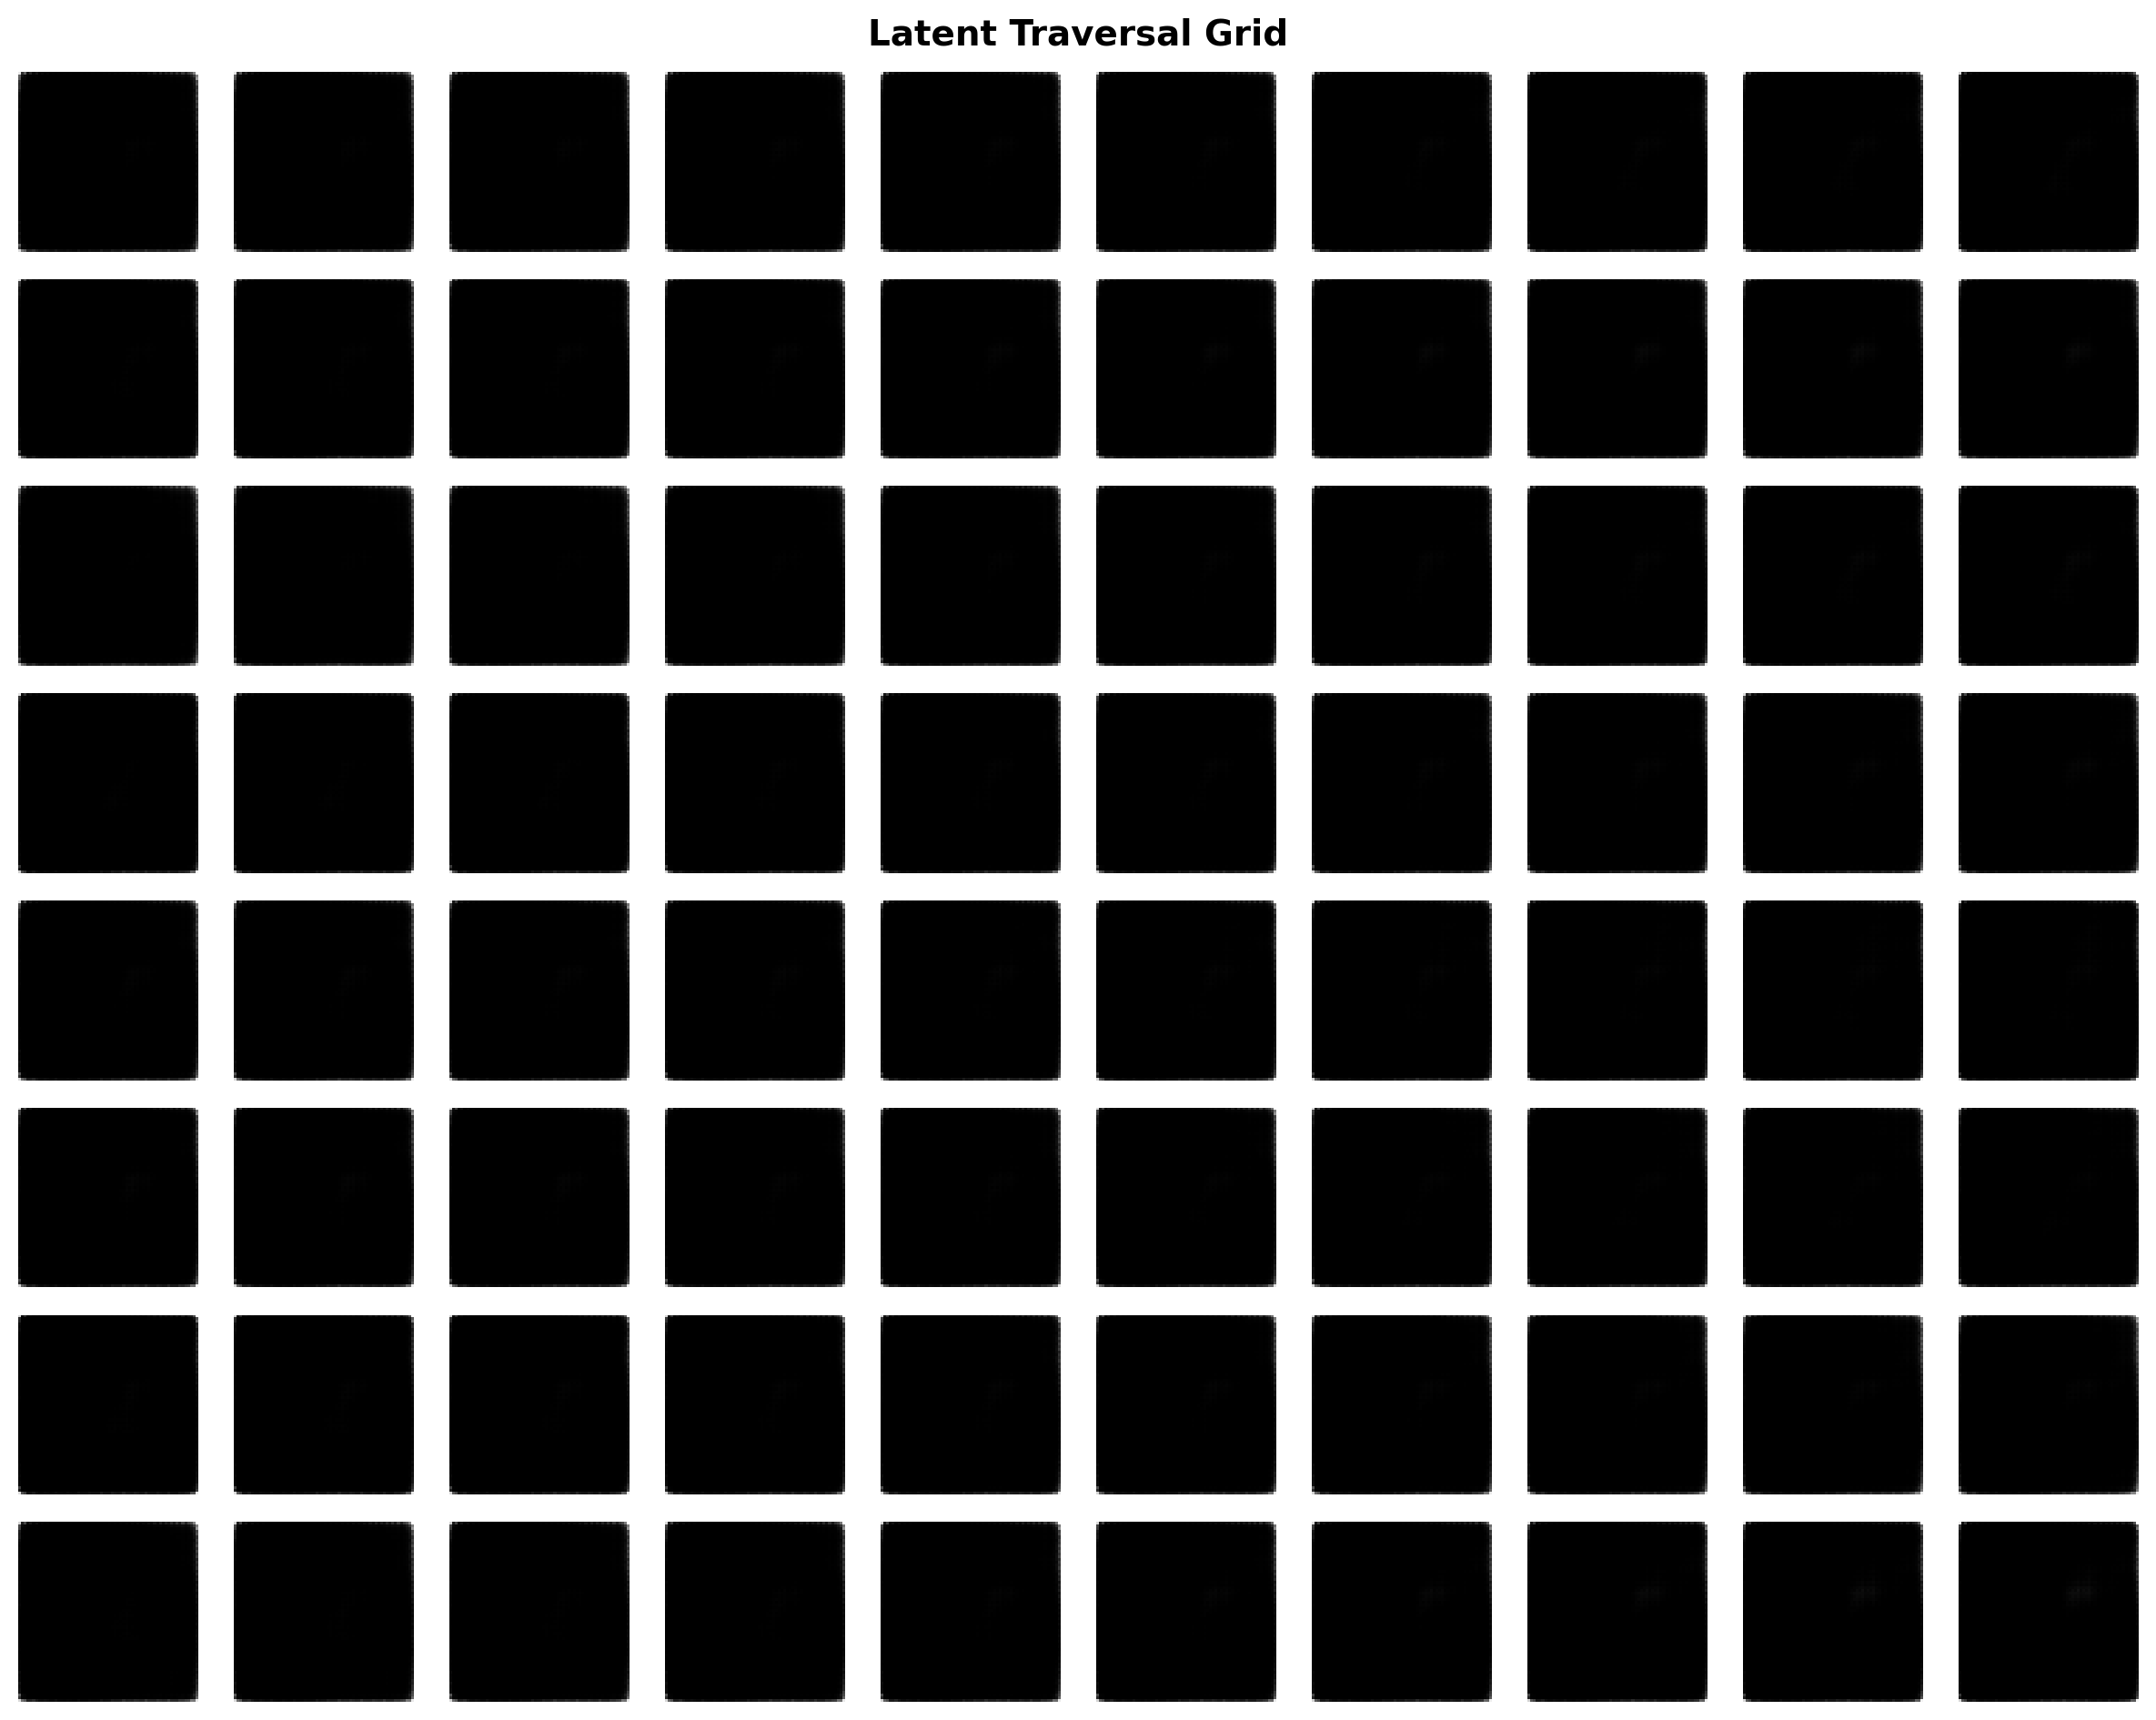
\includegraphics[width=3.5in]{8.png}
\caption{Latent space traversal showing how individual latent dimensions control specific factors of variation. Each row shows variations along one latent dimension while keeping others fixed.}
\label{fig:latent_traversal}
\end{figure}

\begin{figure}[!t]
\centering
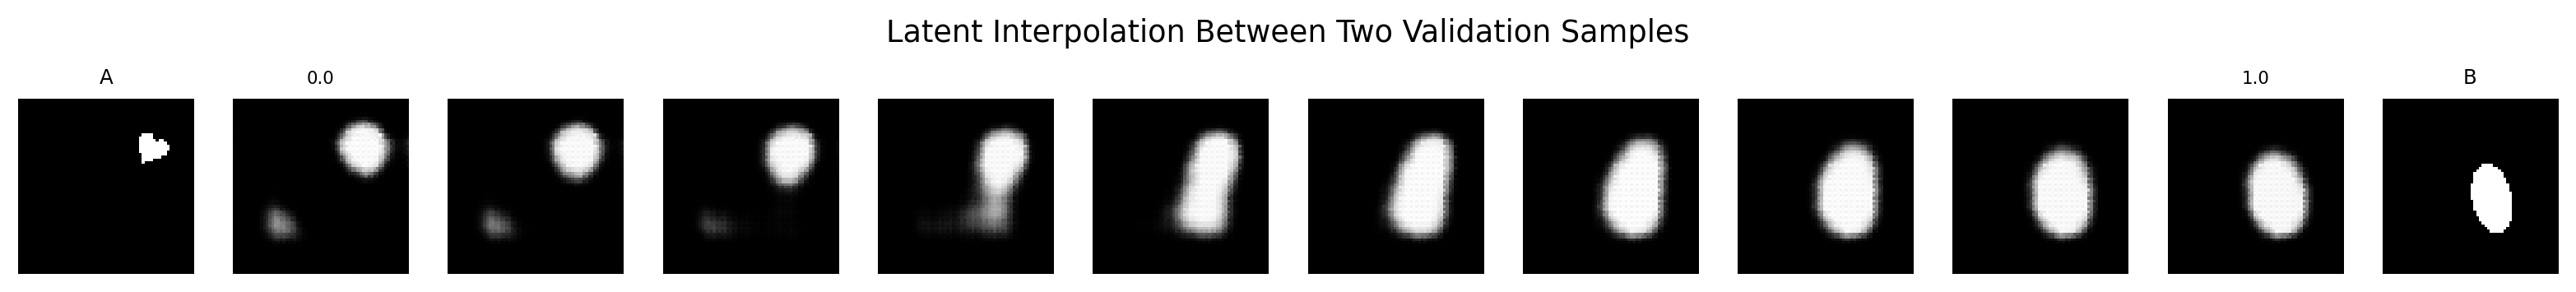
\includegraphics[width=3.5in]{10.png}
\caption{Linear interpolation in latent space between two images. Smooth transitions demonstrate continuity of the learned latent space.}
\label{fig:interpolation}
\end{figure}

\subsection{Training Dynamics}

\begin{figure}[!t]
\centering
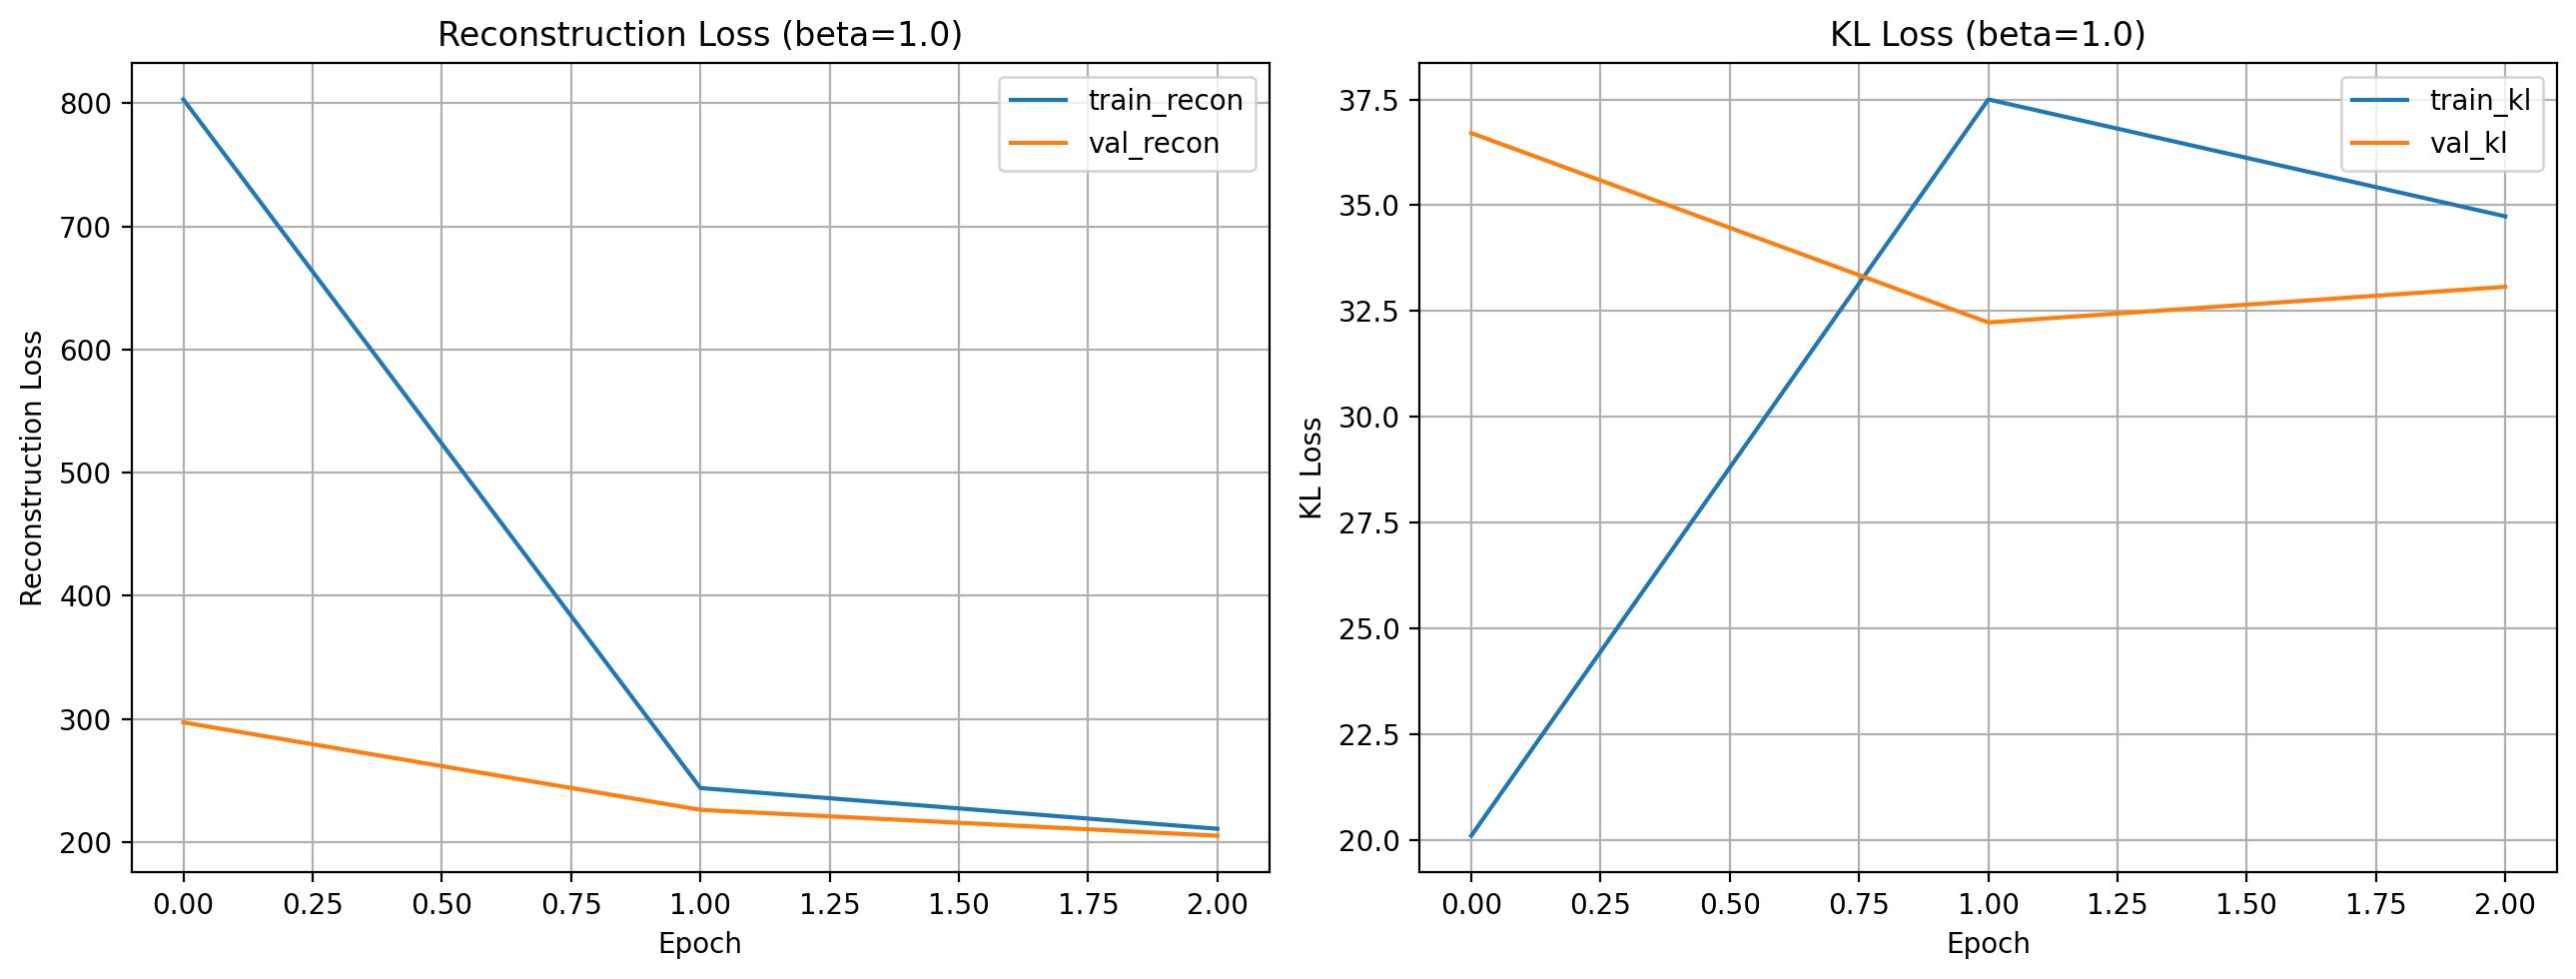
\includegraphics[width=3.5in]{13.png}
\caption{Evolution of loss components during training showing the interplay between reconstruction and KL divergence terms.}
\label{fig:loss_components}
\end{figure}

\begin{figure}[!t]
\centering
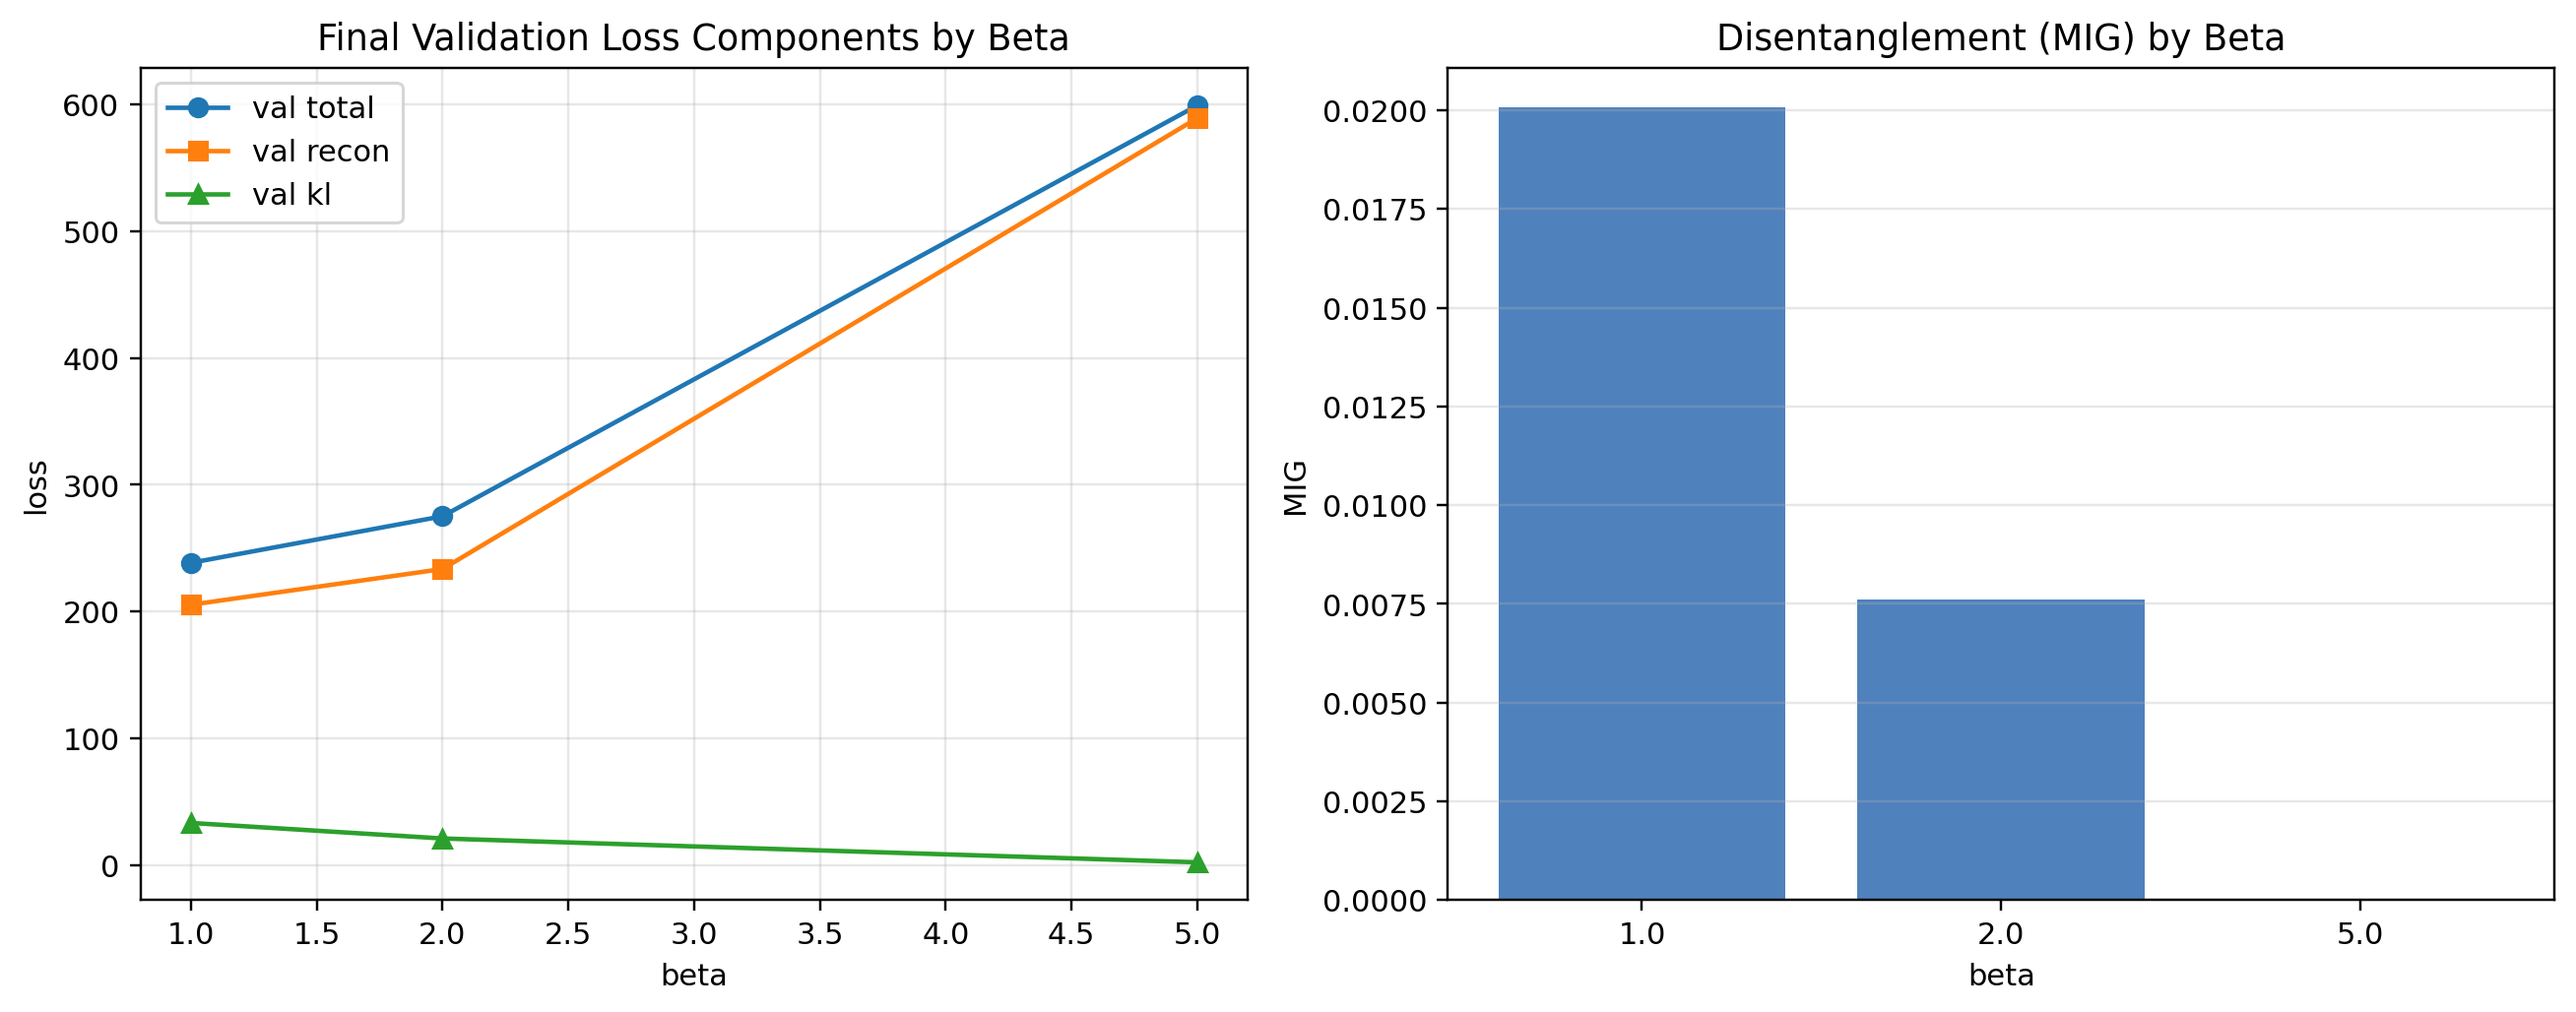
\includegraphics[width=3.5in]{11.png}
\caption{Learning curves comparing different $\beta$ values. Higher $\beta$ leads to slower convergence but better final disentanglement.}
\label{fig:learning_curves}
\end{figure}

\subsection{Qualitative Analysis}

\begin{figure}[!t]
\centering
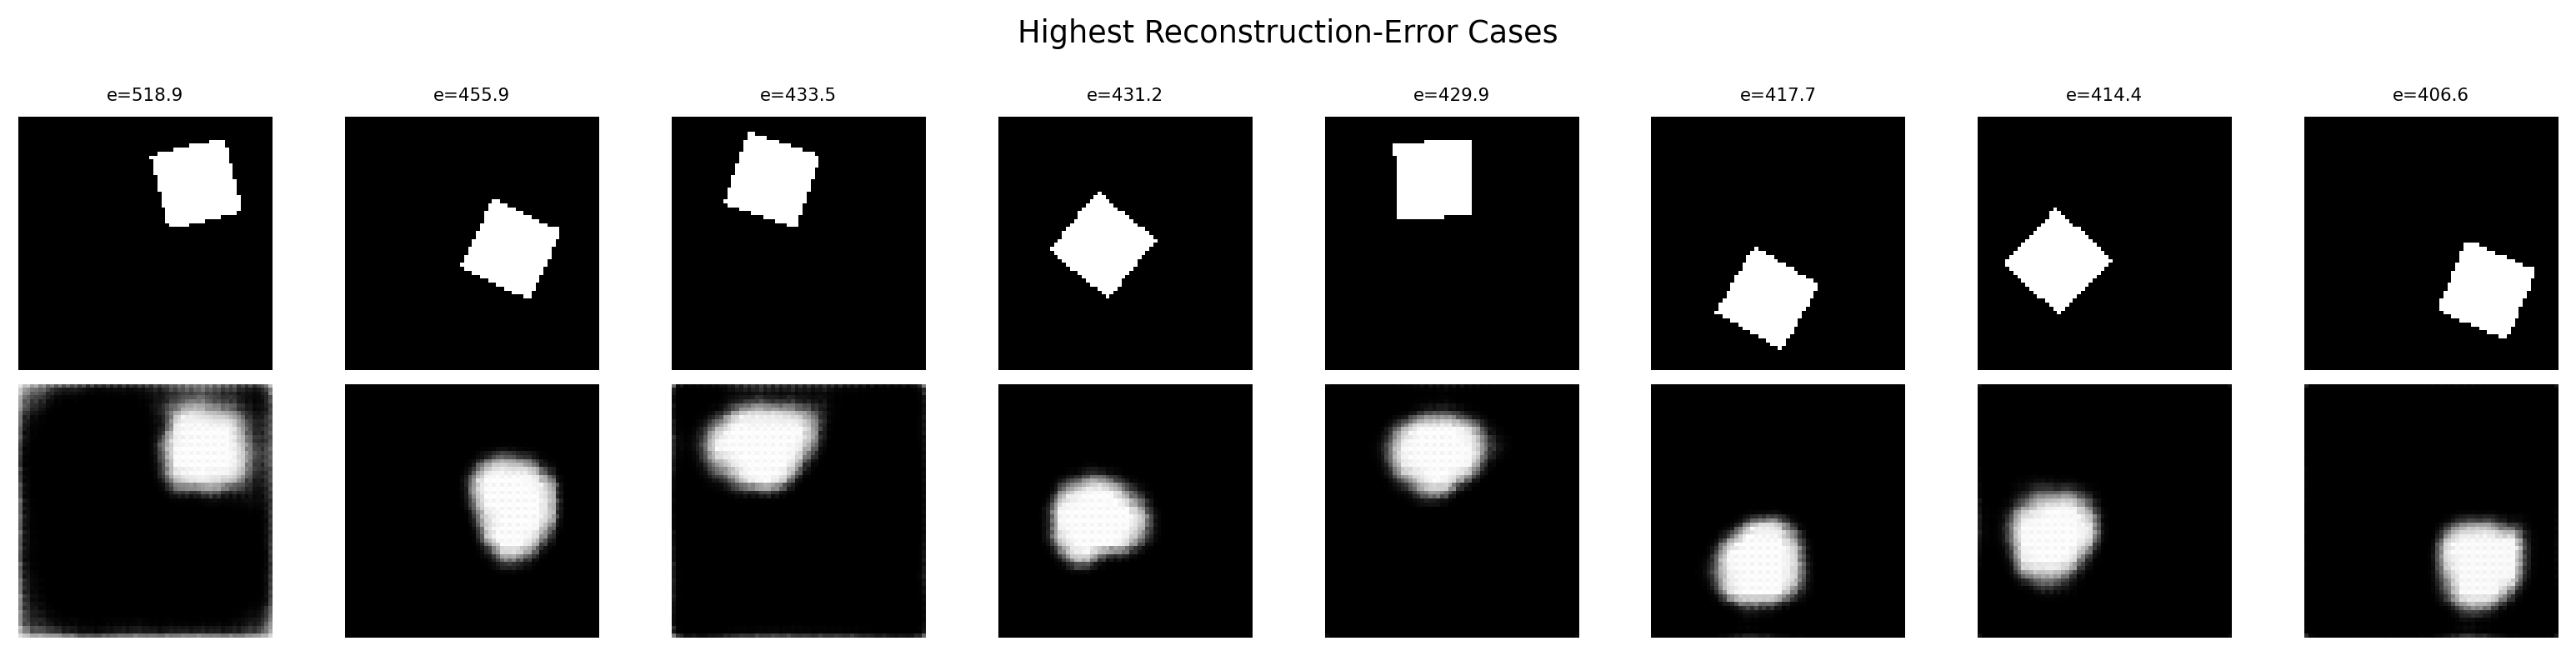
\includegraphics[width=3.5in]{12.png}
\caption{Failure cases showing reconstruction errors. High $\beta$ models struggle with fine details and overlapping shapes.}
\label{fig:failures}
\end{figure}

\section{Course Information}

\subsection{Assignment Details}
\begin{itemize}
    \item \textbf{Course}: Deep Generative Models
    \item \textbf{Instructor}: Dr. Mostafa Tavasoli Pour
    \item \textbf{Institution}: University of Tehran, School of Electrical and Computer Engineering
    \item \textbf{Semester}: Fall 2024
    \item \textbf{Assignment}: Computer Assignment 1
    \item \textbf{Topics}: Probabilistic Graphical Models, Variational Autoencoders
\end{itemize}

\subsection{Acknowledgments}

This implementation builds upon:
\begin{itemize}
    \item PyTorch VAE tutorial by Kingma \& Welling
    \item dSprites dataset by DeepMind
    \item disentanglement\_lib by Google Research
    \item Course materials and lecture notes from Dr. Tavasoli Pour
\end{itemize}

\end{document}
